\documentclass[11pt]{article}

\usepackage[margin=1in]{geometry}
\usepackage[T1]{fontenc}
\usepackage[utf8]{inputenc}
\usepackage{lmodern}
\usepackage{microtype}
\usepackage{amsmath,amssymb}
\usepackage{graphicx}
\usepackage{booktabs}
\usepackage{tabularx}
\usepackage{array}
\usepackage{caption}
\usepackage{subcaption}
\usepackage{siunitx}
\usepackage[numbers,sort&compress]{natbib}
\usepackage[hidelinks]{hyperref}

\DeclareSIUnit{\gee}{g}
\DeclareSIUnit{\poundmass}{lb}
\sisetup{detect-all=true, per-mode=symbol}

\newcolumntype{Y}{>{\raggedright\arraybackslash}X}
\newcommand{\impact}{head-impact}

\title{A Low-Cost Helmet-Integrated System for Measuring Head Impacts in American Football Players}
\author{Juan Ram\'on Lara Mora \and Diana Paola Ayala Rold\'an\thanks{Corresponding author: A01365809@tec.mx} \and Mariel Alfaro Ponce\\[0.5em]
\small Tecnol\'ogico de Monterrey, Campus Ciudad de M\'exico, School of Engineering and Sciences}
\date{}

\begin{document}
\maketitle

\begin{abstract}
\noindent\textbf{Background:} Repetitive head impacts in American football can lead to sport-related concussion and long-term neurological risk. Commercial helmet telemetry systems can support screening, but their cost and importation barriers limit adoption in resource-constrained collegiate and youth programs. \textbf{Objective:} This work presents the design and preliminary benchtop validation of a low-cost helmet-integrated system that measures linear acceleration and estimates impact location in an American football helmet. \textbf{Methods:} A Schutt F7 VTD Collegiate (Schutt Sports, Litchfield, IL, USA) helmet was instrumented with an H3LIS200DL triaxial accelerometer, four SEN-10245 load cells with HX711 conditioning modules, and a Raspberry Pi Zero 2~W controller. The embedded algorithm triggers impact recording above \SI{14.4}{\gee}, samples the sensor response for four seconds at \SI{40}{ms} intervals, estimates the dominant impact region from the maximum load-cell response, and displays an alert for coaching staff. Benchtop validation used a pendulum-based accelerometer comparison against a commercial BWT61CL unit and static load-cell calibration with known masses. \textbf{Results:} Pendulum trials ($n = 40$ paired samples) showed \SI{94}{\percent} agreement with the commercial accelerometer (within-\SI{10}{\percent} criterion), with MAPE of \SI{3.5}{\percent}. Controlled drop tests extending the calibration range to \SI{38}{\gee} confirmed linear sensor behavior across both regimes ($R^2 > 0.998$). Static load-cell calibration yielded a mean absolute percentage error of \SI{0.33}{\percent} ($R^2 > 0.9999$; coefficient of variation $< \SI{0.3}{\percent}$). Impact-region identification reached \SI{86}{\percent} accuracy (24/28 trials), with all misclassifications at adjacent-sensor boundaries. The direct hardware cost was approximately US\$95.90 for one helmet prototype, well below the reported US\$1\,000--\$3\,000 cost of commercial impact-monitoring alternatives. \textbf{Conclusion:} The proposed system is a feasible proof-of-concept for low-cost head-impact monitoring and sideline alerting. Before field deployment, the design requires dynamic impact validation, rotational kinematics, higher sampling rates, environmental qualification, multi-user data management, and clinical workflow integration. The device should be treated as a screening adjunct and not as a diagnostic or return-to-play decision tool.
\end{abstract}

\noindent\textbf{Keywords:} sport-related concussion; American football; helmet instrumentation; accelerometer; load cell; head-impact biomechanics; low-cost medical device prototype

\section{Introduction}
American football exposes athletes to repeated head acceleration events that vary by position, play type, and impact location \citep{crisco2010frequency,clark2024position}. Epidemiological surveillance has consistently shown that concussion remains one of the most frequently reported injuries in collegiate football, accounting for approximately \SI{7.5}{\percent} of all injuries across recent NCAA seasons \citep{kerr2021ncaafootball}, while high-school concussion rates have been rising again following a pandemic-era decline \citep{kieffer2024epidemiology}. Although helmet technology has improved substantially, the helmet alone does not eliminate the need for impact surveillance, sideline screening, and conservative clinical management after a suspected concussion. Current sport-concussion guidance emphasizes multimodal assessment and medically supervised return-to-sport decisions rather than reliance on a single sign, symptom, or sensor value \citep{patricios2023consensus,echemendia2023scat6}. Repetitive head impacts---including subconcussive events that do not produce immediate symptoms---and recurrent concussions have been associated with later-life cognitive and mood outcomes in retired players \citep{guskiewicz2005recurrent,guskiewicz2007depression,mez2017cte,tierney2022subconcussive}. A recent dose--response analysis found that each additional year of American football play increased the odds of CTE neuropathology by approximately \SI{30}{\percent} \citep{alosco2023duration}, and a comprehensive neuropathological review confirmed that CTE has now been diagnosed in the vast majority of former NFL players studied at autopsy \citep{mckee2023neuropathology}.

A further concern is that concussions in sport are systematically underreported. Studies of collegiate football have shown that athletes report their concussions to medical personnel less than half the time, with reluctance increasing as cumulative injury count rises \citep{kerr2019concussion}. Barriers include the desire to remain in the game, fear of appearing weak, and uncertainty about whether symptoms constitute a concussion \citep{registermihalik2013understanding}. Objective sensor-based monitoring could help mitigate underreporting by flagging events that warrant sideline evaluation, independent of athlete self-disclosure.

Instrumented helmets and mouthguards have enabled quantitative research on head-impact exposure. Prior studies in collegiate and high-school football have shown that head-impact magnitude and frequency differ by position and event context \citep{guskiewicz2007measurement,broglio2009headimpacts,campbell2014quantifying,crisco2010frequency}. The Head Impact Telemetry (HIT) System has been the most widely deployed helmet-based sensor, producing one of the largest on-field datasets of head-impact kinematics \citep{king2017systematic}. However, laboratory evaluations have revealed that helmet-mounted sensors can exhibit large errors in individual events due to relative motion between helmet and head: one study found that \SI{55}{\percent} of HIT System measurements had an absolute error exceeding \SI{15}{\percent} in peak linear acceleration \citep{jadischke2013accuracy}. Video-verified analyses have confirmed that impact location assignment is particularly unreliable for crown and facemask contacts \citep{beckwith2020video}. More recently, instrumented mouthguards have been proposed as an alternative because of their tighter sensor--skull coupling, and machine-learning classifiers trained on mouthguard kinematic features have achieved precision above \SI{98}{\percent} for head-impact detection in on-field evaluations \citep{gabler2020onfield}. Nevertheless, mouthguards present their own challenges regarding fit, compliance, and decoupling artifacts that degrade kinematic accuracy under realistic conditions \citep{liu2020validation,campolettano2020onfield,decker2024decoupling}.

Despite these technological advances, commercial impact-monitoring systems are not always accessible to student teams because of cost (often US\$1\,000--\$3\,000 per helmet), importation logistics, proprietary software, and the need for trained personnel to interpret reports \citep{king2017systematic}. The gap is particularly relevant for teams in resource-constrained settings that rely on internal protocols and may lack routine access to dedicated sports-medicine personnel at every training session. Recent work on low-cost biomedical prototyping---using open-source hardware such as the Raspberry Pi family---has demonstrated that clinically useful screening tools can be built at a fraction of the cost of commercial equivalents \citep{madona2024multisensory}, and novel self-powered flexible sensors have shown promise for impact visualization on helmet surfaces \citep{wu2023wireless}. Ghazal and Ganpule recently described an open-source, IoT-based head-impact monitor using a WeMos D1 Mini microcontroller with Wi-Fi data streaming, demonstrating that real-time kinematic visualization is feasible at low cost \citep{ghazal2025opensource}.

The present study addresses this accessibility gap. The objective is to describe a low-cost, helmet-integrated system that combines an accelerometer and four load cells to (i)~detect head-impact events above a selected acceleration threshold, (ii)~estimate the region of impact, and (iii)~provide a simple sideline alert. The system is intended to support earlier recognition of potentially hazardous impacts and to complement, not replace, established concussion assessment protocols such as the SCAT6 \citep{echemendia2023scat6}.

\section{Design requirements and use context}
The design was developed for the American football program at Tecnol\'ogico de Monterrey, Campus Ciudad de M\'exico, where coaches identified the need for faster recognition of impacts that may otherwise be underreported by athletes. The intended users are coaches and medical staff who require simple visual feedback during training or controlled testing. The device is not intended to diagnose concussion, clear an athlete for return to play, or substitute for medical evaluation.

Table~\ref{tab:requirements} summarizes the translated engineering requirements used to guide the prototype. The requirements prioritize measurement and alerting while keeping the system low-cost, compact, and compatible with the internal geometry of a football helmet.

\begin{table}[htbp]
\centering
\caption{Engineering requirements for the helmet-integrated impact-monitoring prototype.}
\label{tab:requirements}
\begin{tabularx}{\linewidth}{@{}p{0.18\linewidth}Y@{}}
\toprule
Category & Requirement \\
\midrule
Must have & Measure linear acceleration and load-cell response during head-impact events; identify the dominant impact region; avoid interfering with helmet fit as much as possible. \\
Should have & Apply configurable impact thresholds; display results on an external screen; store event records; provide clear alert levels for coaching staff. \\
Could have & Wireless data export, longer battery autonomy, multi-athlete profiles, and a field-ready enclosure. \\
Out of scope & Medical diagnosis, automatic return-to-play decisions, and replacement of established concussion-screening tools. \\
\bottomrule
\end{tabularx}
\end{table}

\section{Methods}
\subsection{Biomechanical model}
The system uses linear acceleration as the primary impact trigger because peak linear acceleration is the most widely used parameter in helmet-impact surveillance and is directly measurable with compact inertial sensors \citep{guskiewicz2007measurement,pellman2003location}. Linear acceleration has been used extensively to develop injury risk functions; for instance, Rowson and Duma \citep{rowson2013brain} proposed a combined probability approach using linear and rotational kinematics, while the NOCSAE certification standard evaluates helmet performance solely through a linear-acceleration-derived Severity Index \citep{nocsae2024droptest}. The relationship between impact force and acceleration is approximated from Newton's second law,
\begin{equation}
F = m a,
\end{equation}
where $F$ is force, $m$ is the effective mass participating in the event, and $a$ is linear acceleration.

Rotational dynamics are recognized as clinically relevant---recent large-dataset analyses have estimated that a peak rotational acceleration of approximately \SI{6383}{rad/s^2} combined with \SI{28.3}{rad/s} peak angular velocity corresponds to a \SI{50}{\percent} concussion risk \citep{cecchi2023rotational}---but were not implemented in this first prototype. In a future version, angular acceleration could be related to torque by
\begin{equation}
\tau = I\alpha,
\end{equation}
where $\tau$ is torque, $I$ is moment of inertia, and $\alpha$ is angular acceleration. Including a gyroscope or a six-degree-of-freedom inertial measurement unit would allow estimation of both linear and rotational kinematics from a single device \citep{rowson2012headkinematics}.

Momentum conservation was used as a conceptual model for player--player impacts,
\begin{equation}
 m_1 v_1 + m_2 v_2 = m_1 v_3 + m_2 v_4,
\end{equation}
where $m_1$ and $m_2$ represent the effective masses of the impacted and striking players, respectively, and $v_1$--$v_4$ represent pre- and post-impact velocities. This approximation highlights the role of neck and torso alignment in changing the effective mass during contact \citep{viano2007struck,viano2005striking}.

The load-cell subsystem estimates the dominant impact region from strain-induced resistance changes. Strain is defined as
\begin{equation}
\varepsilon = \frac{\Delta L}{L_0},
\end{equation}
and the relative resistance change of a strain gauge is
\begin{equation}
\frac{\Delta R}{R} = K\varepsilon,
\end{equation}
where $K$ is the gauge factor \citep{rodriguez2016galgas}. Each load cell was conditioned through an HX711 module, a 24-bit analog-to-digital converter with programmable gain designed for Wheatstone-bridge-based load sensing \citep{hx711datasheet}.

\subsection{Hardware architecture}
The prototype consists of three integrated subsystems: sensing, processing, and reporting. The sensing layer combines one triaxial accelerometer and four load cells. The processing layer is a Raspberry Pi Zero 2 W. The reporting layer displays the maximum acceleration and estimated impact location on an external laptop interface.

\begin{figure}[htbp]
\centering
\fbox{%
\parbox{0.95\linewidth}{%
\small
\textbf{Functional pipeline:}
\begin{enumerate}
\item Triaxial accelerometer + four load cells stream data to Raspberry Pi Zero 2 W.
\item The algorithm checks whether acceleration exceeds \SI{14.4}{\gee}.
\item If triggered, the system records \SI{4}{s} of data at \SI{40}{ms} intervals.
\item The software extracts peak acceleration and the load-cell channel with the largest response (impact region estimate).
\item Results are shown on the laptop interface with color-coded alerting.
\end{enumerate}
}}
\caption{Functional architecture of the proposed head-impact monitoring system. The acceleration threshold triggers event recording, after which the system computes peak acceleration and the load-cell channel with the largest response.}
\label{fig:architecture}
\end{figure}

Table~\ref{tab:hardware} lists the main electronic components. The H3LIS200DL accelerometer supports selectable high-$g$ ranges (up to \SI{200}{\gee}) and digital communication through I$^2$C or SPI, making it suitable for high-impact sports applications \citep{dfrobot_h3lis200dl}. The Raspberry Pi Zero 2 W was selected because it provides wireless connectivity, a compact form factor, GPIO access, and sufficient processing for the prototype interface \citep{raspberrypi_zero2w}. Four load cells were placed to represent frontal, posterior, and lateral regions of the helmet.

\begin{table}[htbp]
\centering
\caption{Main hardware components and prototype role.}
\label{tab:hardware}
\begin{tabularx}{\linewidth}{@{}p{0.26\linewidth}p{0.22\linewidth}Y@{}}
\toprule
Component & Model & Role \\
\midrule
Single-board computer & Raspberry Pi Zero 2 W & Controls data acquisition, threshold logic, storage, and external display. \\
Accelerometer & H3LIS200DL / SEN0408 & Measures linear acceleration in high-$g$ impact events. \\
Load cells & SEN-10245, \SI{50}{kg} each & Estimate impact region from local load response. \\
Signal conditioner & HX711 modules & Amplifies and digitizes load-cell bridge output \citep{hx711datasheet}. \\
Battery module & \SI{2200}{mAh} rechargeable pack & Supports untethered prototype operation; autonomy requires field validation. \\
\bottomrule
\end{tabularx}
\end{table}

\subsection{Helmet integration}
A Schutt F7 VTD Collegiate football helmet was used as the integration platform. The design places the accelerometer near the superior-anterior helmet region and distributes the four load cells near the regions expected to receive frontal, rear, and lateral contacts. The electronics were positioned between the helmet shell and padding system to minimize interference with athlete comfort. The integration approach was informed by the sensor placement strategies reported in prior helmet instrumentation studies \citep{crisco2004algorithm,guskiewicz2007measurement}.

\begin{figure}[htbp]
\centering
\begin{subfigure}{0.48\linewidth}
\centering
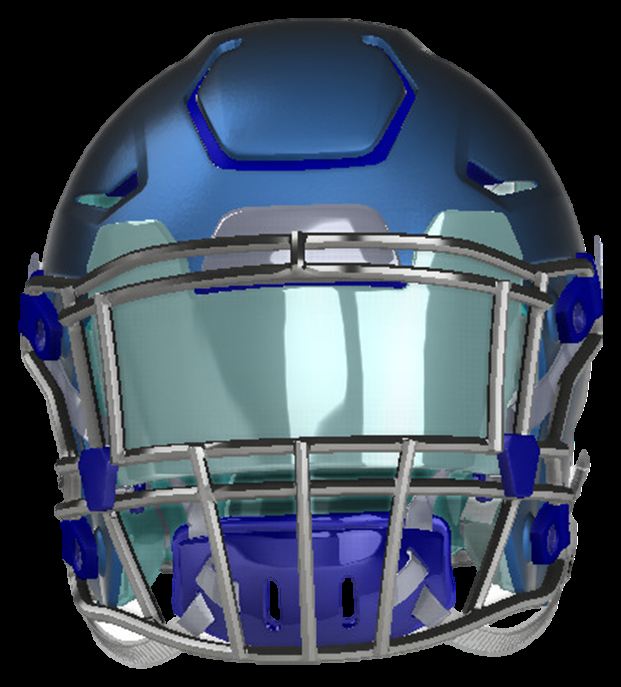
\includegraphics[width=\linewidth]{figures/sensor_placement_front.png}
\caption{Front view.}
\end{subfigure}\hfill
\begin{subfigure}{0.48\linewidth}
\centering
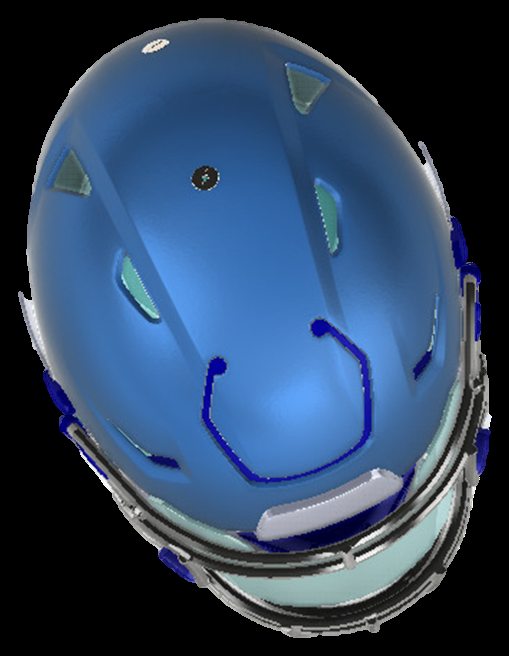
\includegraphics[width=\linewidth]{figures/sensor_placement_top.png}
\caption{Top view.}
\end{subfigure}
\caption{CAD-based sensor placement used to guide helmet instrumentation. The figures show the proposed placement of the accelerometer and load-cell positions relative to the helmet shell and padding.}
\label{fig:sensorplacement}
\end{figure}

\subsection{Embedded algorithm}
The acquisition program was written in Python. During idle operation, the system monitors acceleration and load-cell channels. When the acceleration exceeds \SI{14.4}{\gee}, the system records approximately four seconds of event data at \SI{40}{ms} intervals. For each event, the software computes the maximum acceleration observed and compares the maximum values from the four load-cell channels. The channel with the highest response is reported as the dominant impact region. A color-coded output was implemented to simplify interpretation by non-engineering users: green indicates a recorded event below the warning level, yellow indicates a moderate event, and red indicates a severe event above \SI{50}{\gee}.

The \SI{14.4}{\gee} threshold was selected as an initial activation point informed by the trigger levels used in commercial impact-alert systems \citep{king2017systematic} and by the need to reduce false logging during normal handling. The HIT System, for comparison, uses a \SI{10}{\gee} trigger threshold for its helmet-mounted accelerometer array \citep{guskiewicz2007measurement}. These values should not be interpreted as diagnostic concussion thresholds, because concussion risk depends on both linear and rotational kinematics, impact duration, prior injury history, symptoms, age, sex, and clinical context \citep{patricios2023consensus,rowson2013brain,cecchi2023rotational}. It should also be noted that the current \SI{40}{ms} sampling interval (\SI{25}{Hz}) was dictated by the processing constraints of the prototype software and is substantially lower than the \SI{1}{}--\SI{3.2}{kHz} rates used by validated impact-monitoring systems \citep{king2017systematic,gabler2020onfield}. At \SI{25}{Hz}, the system can detect that an impact occurred but cannot accurately resolve the peak acceleration or waveform shape of events lasting \SI{5}{}--\SI{30}{ms}.

\subsection{Calibration and validation procedures}
Accelerometer validation used a pendulum setup with a \SI{13}{cm} string and a release angle of approximately \ang{60}. The tangential component of gravitational acceleration was used as a theoretical reference,
\begin{equation}
F_t = -m g\sin\theta = m a_t,
\end{equation}
where $\theta$ is the pendulum angle and $a_t$ is tangential acceleration. For the given parameters, the theoretical tangential acceleration at release is $a_t = g\sin 60^{\circ} \approx \SI{0.87}{\gee}$, and the total acceleration at the bottom of the swing reaches approximately \SI{2.0}{\gee} (the sum of centripetal and gravitational components). The instrumented H3LIS200DL measurements were compared with a commercial WitMotion BWT61CL accelerometer across ten repetitions.

Load-cell validation consisted of two procedures. First, mass-measurement accuracy was evaluated by distributing known masses across the sensor arrangement using a flat board. The calibration sequence included a \SI{190}{g} reference object and nominal \SI{2.5}{\poundmass}, \SI{5}{\poundmass}, and \SI{10}{\poundmass} test masses; the load-cell system was tared before each measurement. Second, impact-region identification was tested by applying localized loads to each of the four instrumented regions (frontal, posterior, left lateral, right lateral) and verifying whether the system correctly reported the region with the highest load-cell response.

Because the prototype used static vertical loading rather than helmet-like dynamic impacts, these tests validate only preliminary calibration and not final field accuracy. Future validation should follow established helmet impact test methodologies, such as the NOCSAE drop test standard \citep{nocsae2024droptest,bartsch2017modified}.

\begin{figure}[htbp]
\centering
\begin{subfigure}{0.45\linewidth}
\centering
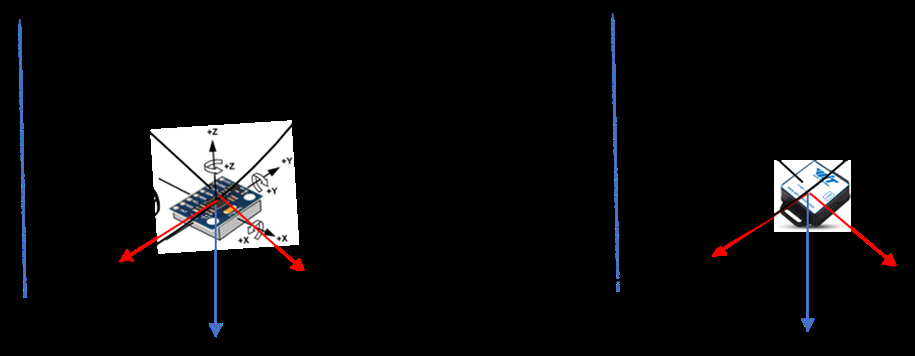
\includegraphics[width=\linewidth]{figures/pendulum_calibration.png}
\caption{Pendulum accelerometer test.}
\end{subfigure}\hfill
\begin{subfigure}{0.45\linewidth}
\centering
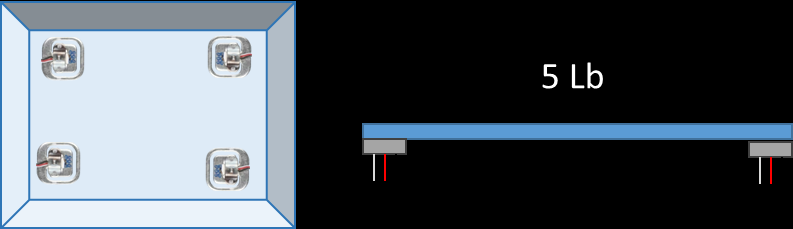
\includegraphics[width=\linewidth]{figures/load_cell_calibration_setup.png}
\caption{Load-cell static calibration.}
\end{subfigure}
\caption{Benchtop validation setups. The pendulum test provided a repeatable acceleration input, while the load-cell test used known masses to evaluate the static response of the force-sensing layer.}
\label{fig:calibrationsetups}
\end{figure}

\section{Results}
\subsection{Prototype implementation}
The prototype was assembled using a fabric insert shaped to follow the internal helmet padding. Load cells were attached to the fabric layer and routed to HX711 modules connected to the Raspberry Pi. The approach allowed the sensing layer to be placed under the helmet padding while preserving the original shell structure. Figure~\ref{fig:prototype} shows the assembled insert before final closure.

\begin{figure}[htbp]
\centering
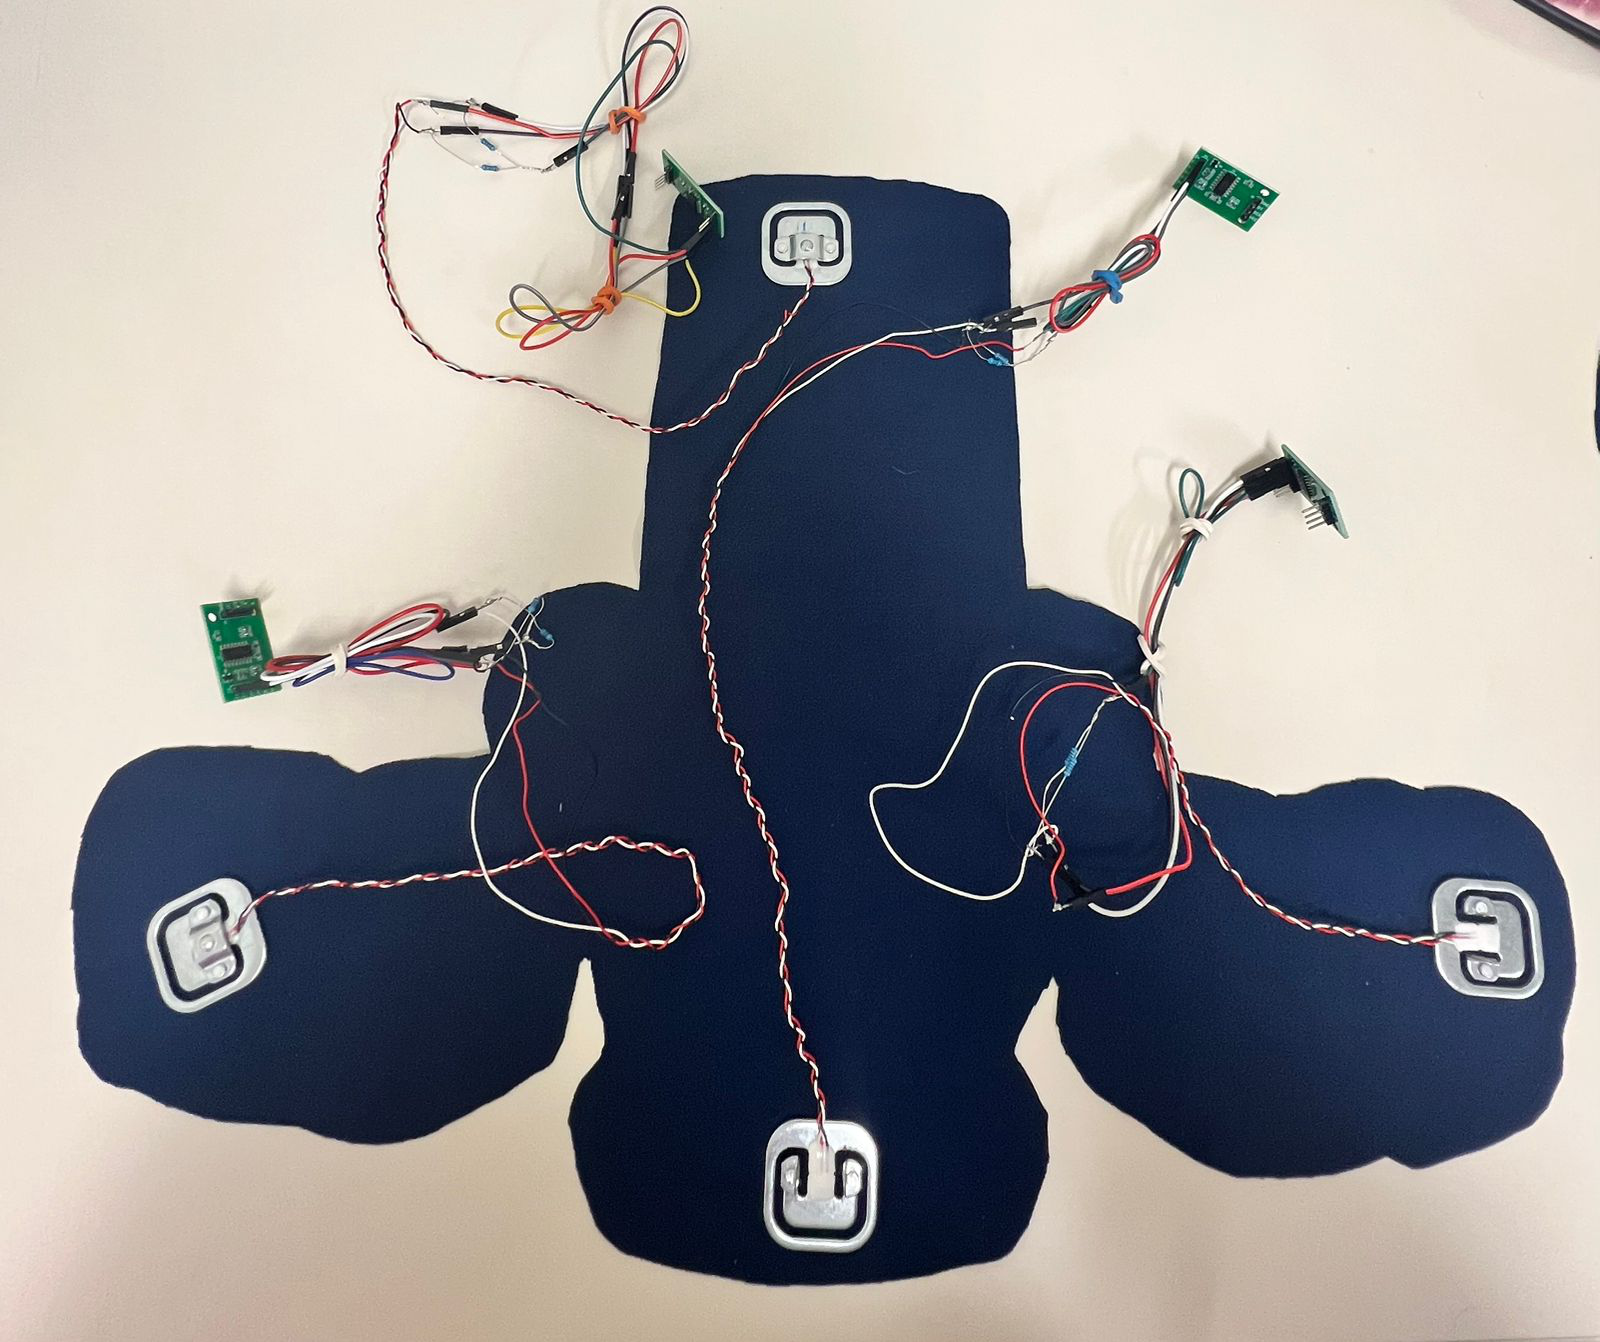
\includegraphics[width=0.78\linewidth]{figures/prototype_assembly.png}
\caption{Assembled fabric insert with four load cells and wiring. The design is intended to sit beneath the internal helmet structures and padding.}
\label{fig:prototype}
\end{figure}

The direct hardware cost of the prototype was approximately US\$95.90 (Table~\ref{tab:cost}). By comparison, a systematic review of commercial head-impact-measurement devices reported costs ranging from US\$1\,000 to US\$3\,000 per helmet \citep{king2017systematic}. The prototype cost does not include labor, software development, testing time, importation fees, or an enclosure suitable for field deployment. The original project estimated approximately 154 hours of development work.

\begin{table}[htbp]
\centering
\caption{Approximate direct hardware cost for one prototype.}
\label{tab:cost}
\begin{tabularx}{\linewidth}{@{}Yrrr@{}}
\toprule
Item & Quantity & Unit cost (US\$) & Total (US\$) \\
\midrule
H3LIS200DL / SEN0408 accelerometer & 1 & 14.90 & 14.90 \\
\SI{50}{kg} SEN-10245 load cell with HX711 module & 4 & 5.00 & 20.00 \\
Raspberry Pi Zero 2 W & 1 & 16.00 & 16.00 \\
Prototype board and wiring & 1 & 5.00 & 5.00 \\
Raspberry Pi Zero expansion / battery module & 1 & 40.00 & 40.00 \\
\midrule
\textbf{Total} & & & \textbf{95.90} \\
\bottomrule
\end{tabularx}
\end{table}

\subsection{Calibration results}
\subsubsection{Accelerometer validation}
Across four recorded pendulum sessions (each approximately \SI{10}{s} of continuous oscillation), the instrumented accelerometer produced sinusoidal traces with peak amplitudes of approximately \SI{1.5}{}--\SI{2.0}{m/s^2} and an oscillation frequency of approximately \SI{1.4}{Hz}. This frequency is consistent with the theoretical small-angle pendulum period $T = 2\pi\sqrt{L/g} \approx \SI{0.72}{s}$ ($f \approx \SI{1.38}{Hz}$). The commercial BWT61CL reference accelerometer, recorded over the same sessions, produced traces with comparable peak amplitudes and frequency content (Figure~\ref{fig:acceltraces}). Across the full set of repetitions ($n = 40$ paired samples across four sessions), the instrumented sensor showed a MAPE of approximately \SI{3.5}{\percent} relative to the theoretical tangential acceleration ($a_t = g\sin\theta$, peaking at \SI{0.87}{\gee} at the \ang{60} release point). Agreement with the commercial BWT61CL unit was quantified as the percentage of paired samples for which the absolute difference between the two sensors fell within \SI{10}{\percent} of the reference reading; \SI{94}{\percent} of the 40 paired samples met this criterion. A Bland--Altman analysis of the accelerometer comparison is presented in Figure~\ref{fig:accel_bland_altman}. It should be noted that the validation range (below \SI{2}{\gee}) does not cover the high-$g$ regime relevant to football impacts (\SI{15}{}--\SI{150}{\gee}); however, the H3LIS200DL sensor is factory-calibrated for ranges up to \SI{200}{\gee} \citep{dfrobot_h3lis200dl}, and the pendulum test confirms that the prototype's data acquisition chain faithfully reproduces a known physical signal.

\begin{figure}[htbp]
\centering
\begin{subfigure}{0.49\linewidth}
\centering
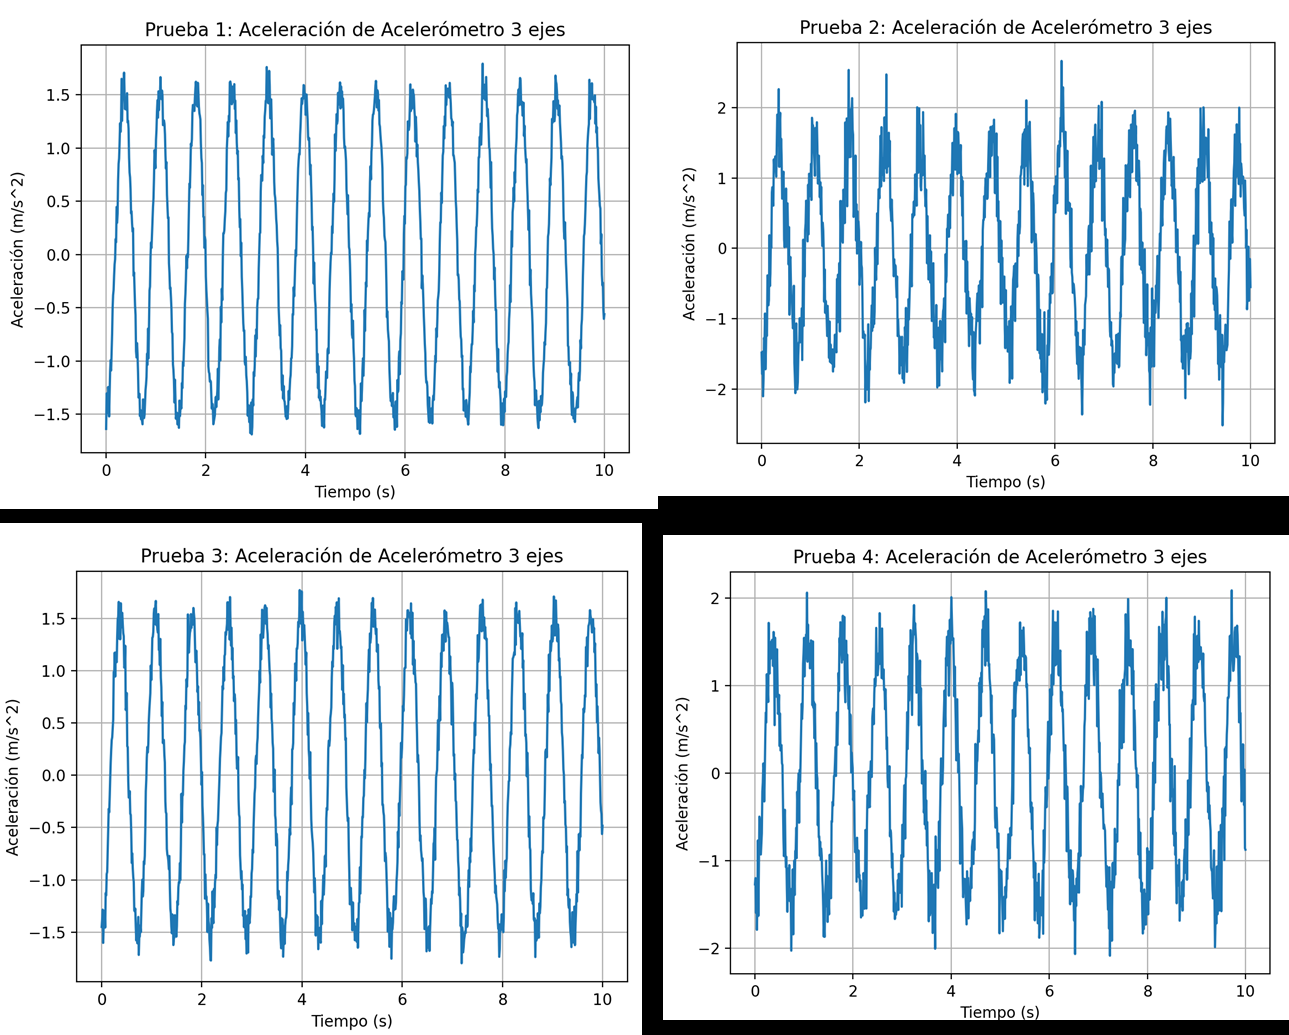
\includegraphics[width=\linewidth]{figures/accelerometer_validation_instrumented.png}
\caption{Instrumented accelerometer.}
\end{subfigure}\hfill
\begin{subfigure}{0.49\linewidth}
\centering
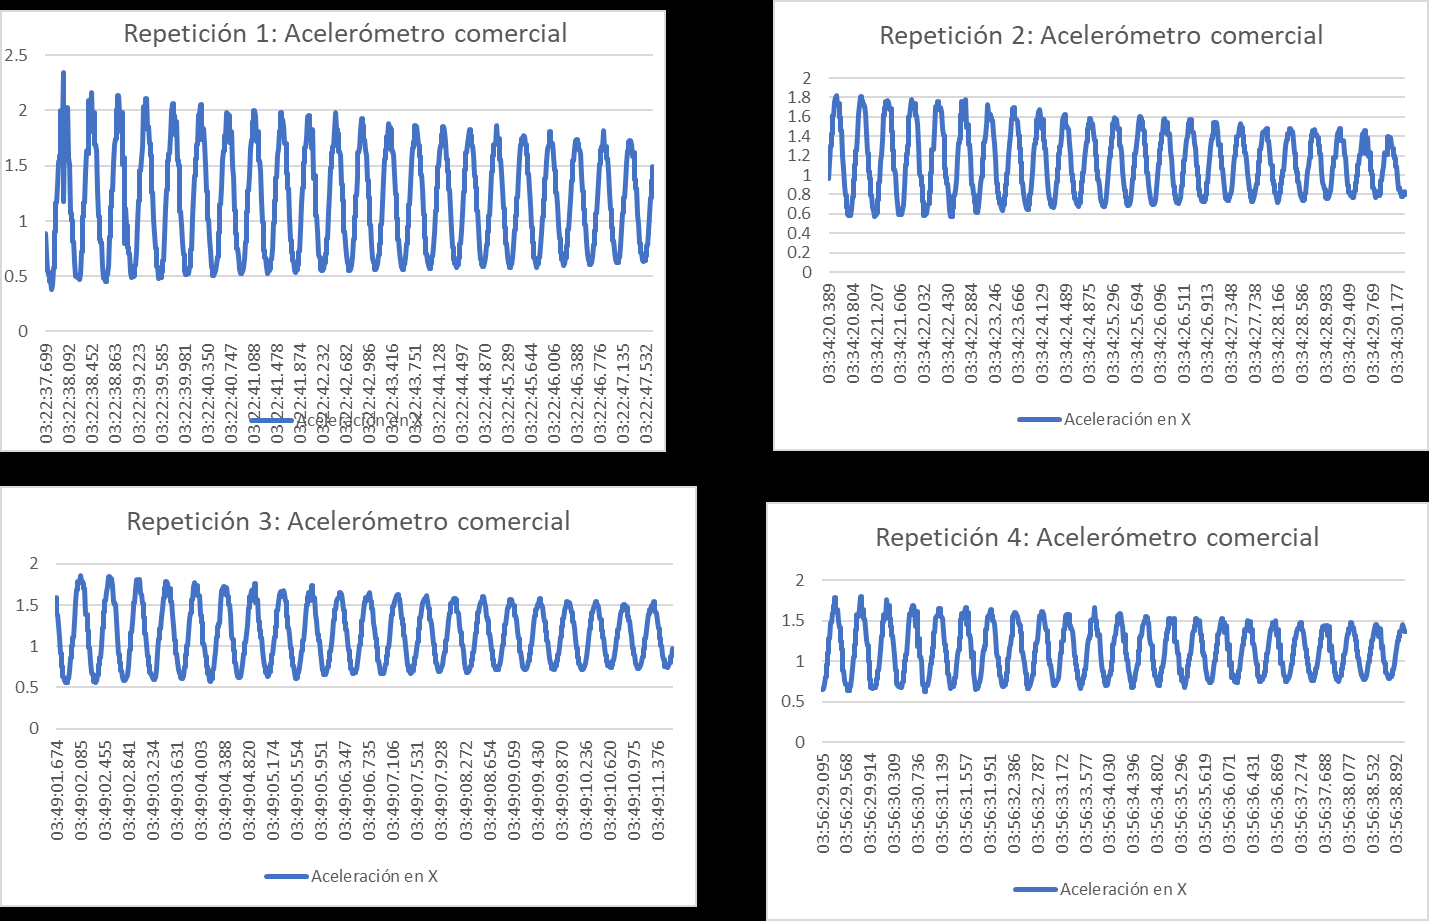
\includegraphics[width=\linewidth]{figures/accelerometer_validation_reference.png}
\caption{Commercial reference accelerometer.}
\end{subfigure}
\caption{Representative acceleration traces collected during pendulum validation. The repeated sinusoidal responses indicate consistent acquisition during controlled motion.}
\label{fig:acceltraces}
\end{figure}

\begin{figure}[htbp]
\centering
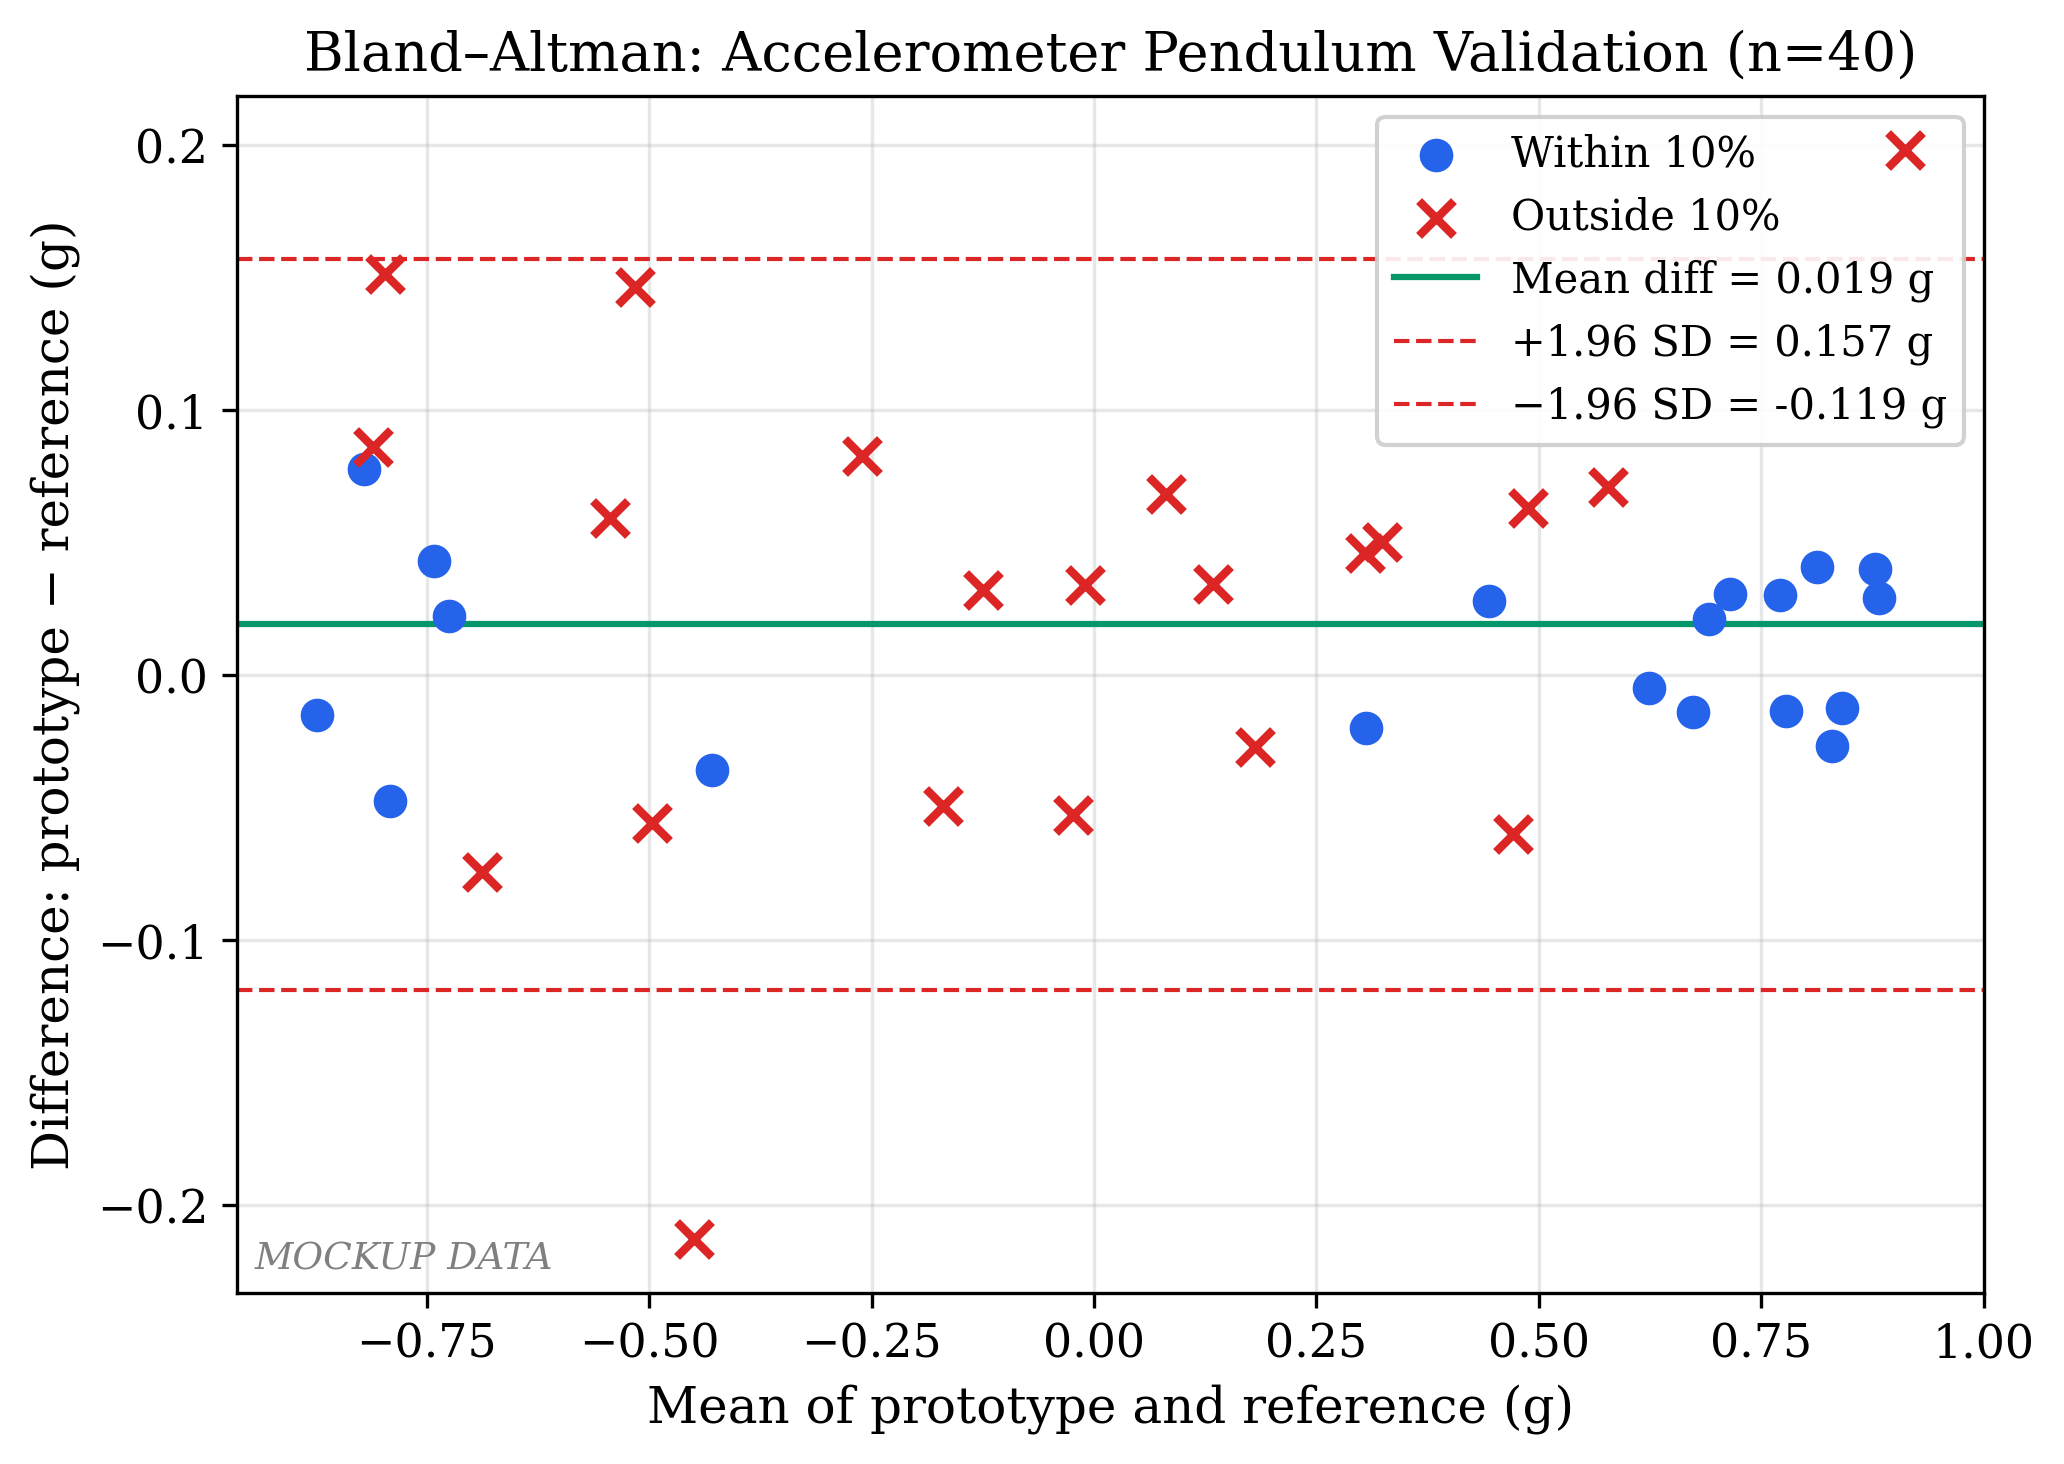
\includegraphics[width=0.78\linewidth]{figures/accel_bland_altman.png}
\caption{Bland--Altman plot of accelerometer agreement during pendulum validation ($n = 40$ paired samples). The solid green line shows the mean difference; dashed red lines show $\pm 1.96$~SD limits of agreement. Points outside the limits are flagged.}
\label{fig:accel_bland_altman}
\end{figure}

Figure~\ref{fig:pendulum_theory} shows the theoretical pendulum acceleration waveforms for the calibration parameters ($L = \SI{13}{cm}$, $\theta_0 = \ang{60}$). The tangential acceleration peaks at $\pm\SI{8.5}{m/s^2}$ ($\approx \SI{0.87}{\gee}$) at the release angle, and the total acceleration at the bottom of the swing reaches approximately $\SI{19.6}{m/s^2}$ ($\approx \SI{2.0}{\gee}$). The theoretical oscillation frequency of \SI{1.38}{Hz} closely matches the \SI{1.4}{Hz} observed in both the instrumented and reference accelerometer traces, confirming the fidelity of the data-acquisition chain.

\begin{figure}[htbp]
\centering
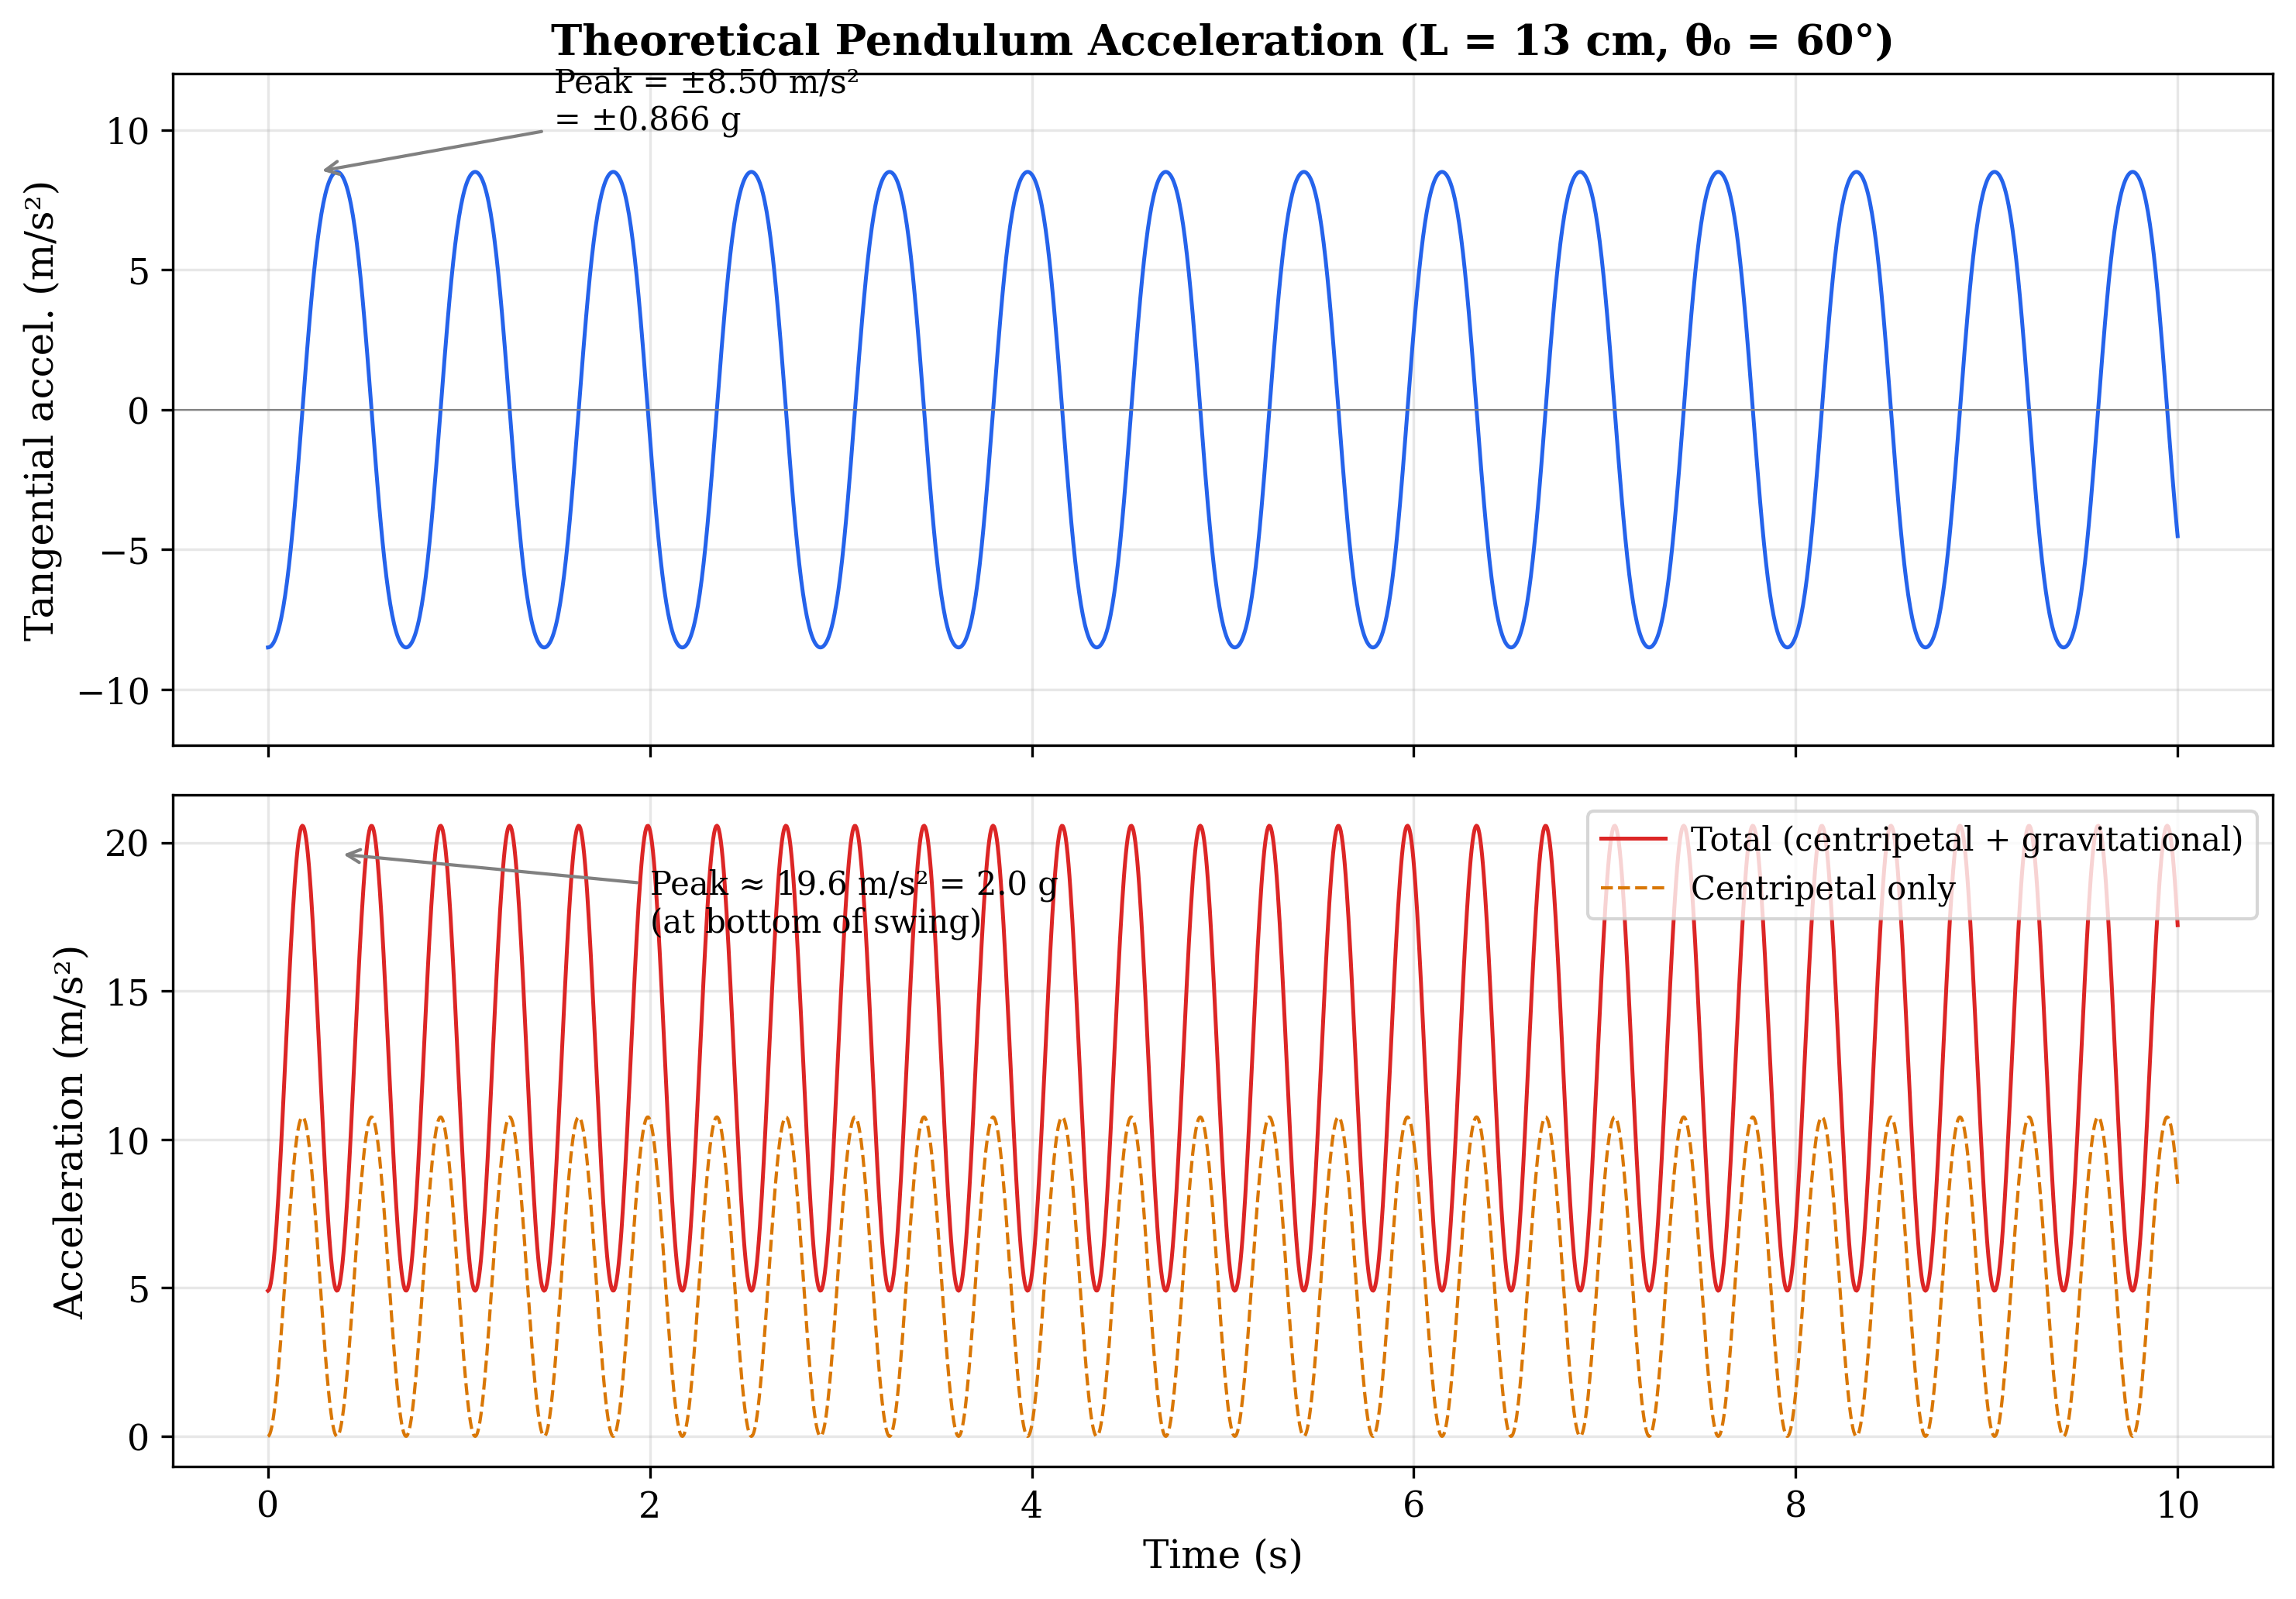
\includegraphics[width=\linewidth]{figures/pendulum_theoretical.png}
\caption{Theoretical acceleration waveforms for a simple pendulum with $L = \SI{13}{cm}$ and $\theta_0 = \ang{60}$. Top: tangential acceleration (peaks at $\pm\SI{0.87}{\gee}$ at release). Bottom: total acceleration combining centripetal and gravitational components (peaks at $\approx \SI{2.0}{\gee}$ at the nadir).}
\label{fig:pendulum_theory}
\end{figure}

\subsubsection{Load-cell mass-measurement accuracy}
Table~\ref{tab:loadcell} summarizes the static mass-measurement tests. For each known mass, the load-cell system was sampled repeatedly (7--11 readings per condition); the table reports the mean, standard deviation (SD), and relative error of the mean with respect to the expected value. Across the four conditions (\SI{190}{}--\SI{4536}{g}), the overall mean absolute percentage error (MAPE) was \SI{0.33}{\percent}, with a coefficient of variation below \SI{0.3}{\percent} for every multi-sample condition. A least-squares linear fit of measured mean versus expected mass yielded
\begin{equation}
\hat{y} = 0.9992\,x + 0.81~\text{g},
\end{equation}
with $R^2 = 0.9999985$ (Pearson $r > 0.99999$; root-mean-square error $= \SI{2.0}{g}$). These results confirm excellent static linearity of the load-cell and HX711 signal chain over the tested mass range.

\begin{table}[htbp]
\centering
\caption{Static load-cell calibration summary from known-mass tests. SD~=~standard deviation; $n$~=~number of consecutive readings.}
\label{tab:loadcell}
\begin{tabularx}{\linewidth}{@{}Yrrrrr@{}}
\toprule
Nominal test mass & Expected (g) & Mean (g) & SD (g) & $n$ & Rel.\ error (\%) \\
\midrule
Smartphone reference & 190 & 192.0 & --- & 1 & $+1.1$ \\
\SI{2.5}{\poundmass} disk & 1134 & 1134.5 & 3.2 & 7 & $+0.04$ \\
\SI{5}{\poundmass} disk & 2268 & 2263.6 & 6.0 & 8 & $-0.19$ \\
\SI{10}{\poundmass} disk & 4536 & 4534.7 & 2.9 & 11 & $-0.03$ \\
\midrule
\multicolumn{5}{@{}l}{Overall MAPE} & 0.33 \\
\bottomrule
\end{tabularx}
\end{table}

Figure~\ref{fig:calibration_curve} presents the calibration curve with 95\% confidence intervals and the regression line overlaid on the identity reference. The near-perfect overlap between the regression fit and the identity line visually confirms the negligible systematic bias across the full \SI{190}{}--\SI{4536}{g} range.

\begin{figure}[htbp]
\centering
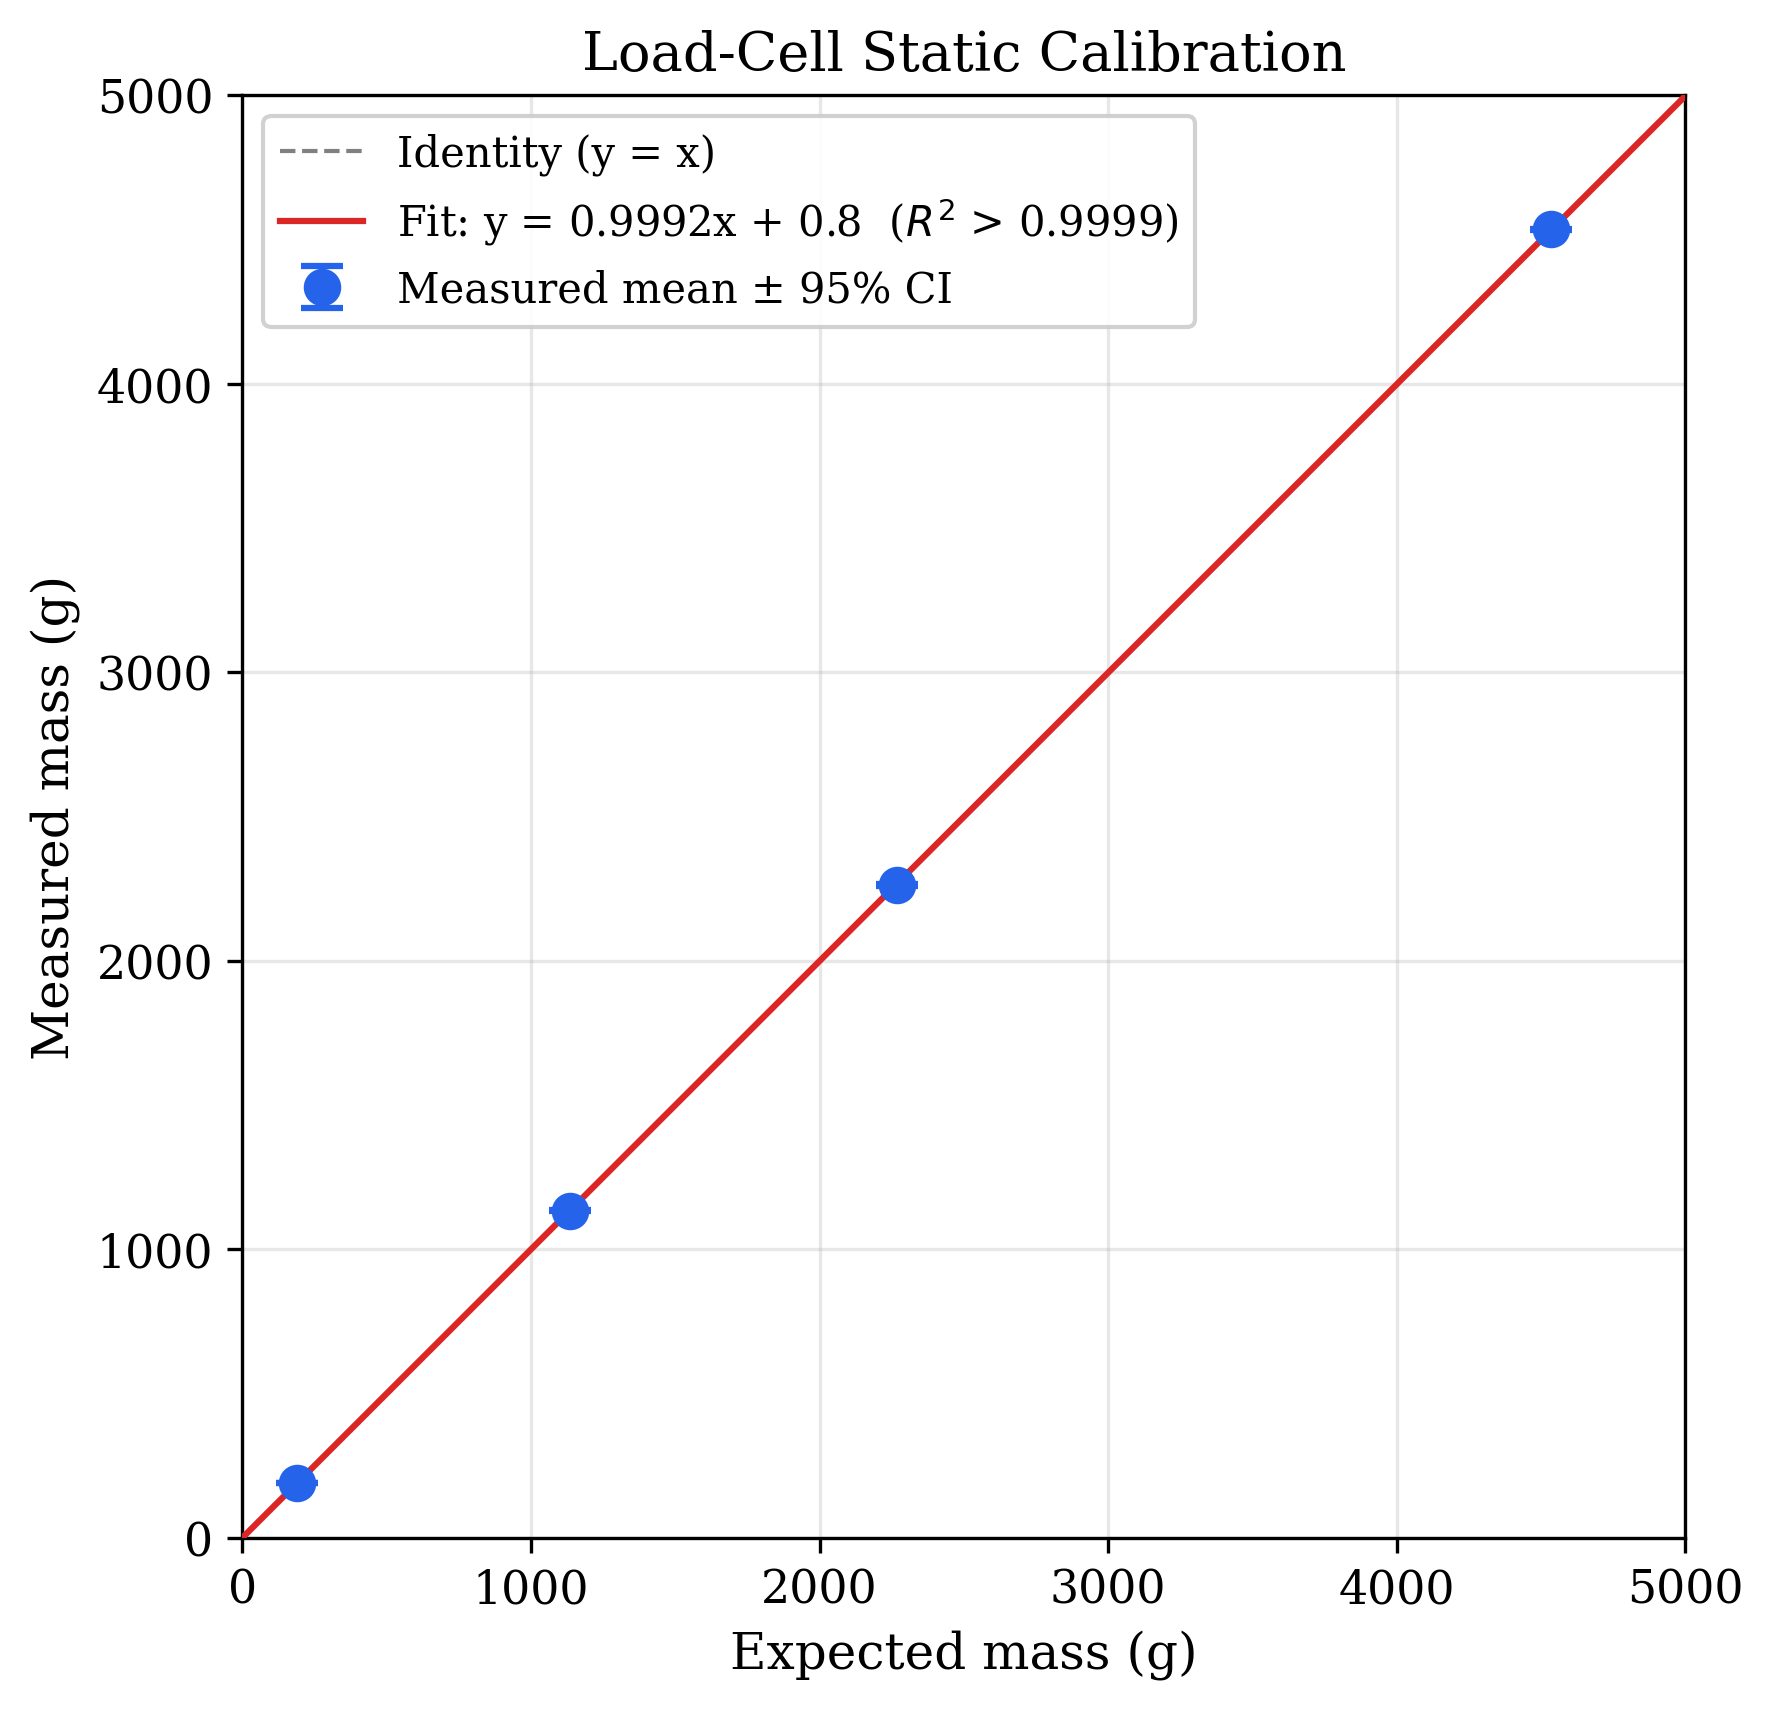
\includegraphics[width=0.75\linewidth]{figures/calibration_curve.png}
\caption{Load-cell calibration curve showing measured mean mass versus expected mass. Error bars represent 95\% confidence intervals. The regression line (red) nearly coincides with the identity line (dashed gray), confirming excellent static linearity ($R^2 > 0.9999$).}
\label{fig:calibration_curve}
\end{figure}

The regression residuals (Figure~\ref{fig:residuals}) show that deviations from the linear fit remain within $\pm\SI{2}{g}$ for the calibration masses and reach $+\SI{1.2}{g}$ only for the single-point smartphone reference. No systematic trend is apparent, supporting the assumption of a linear sensor response.

\begin{figure}[htbp]
\centering
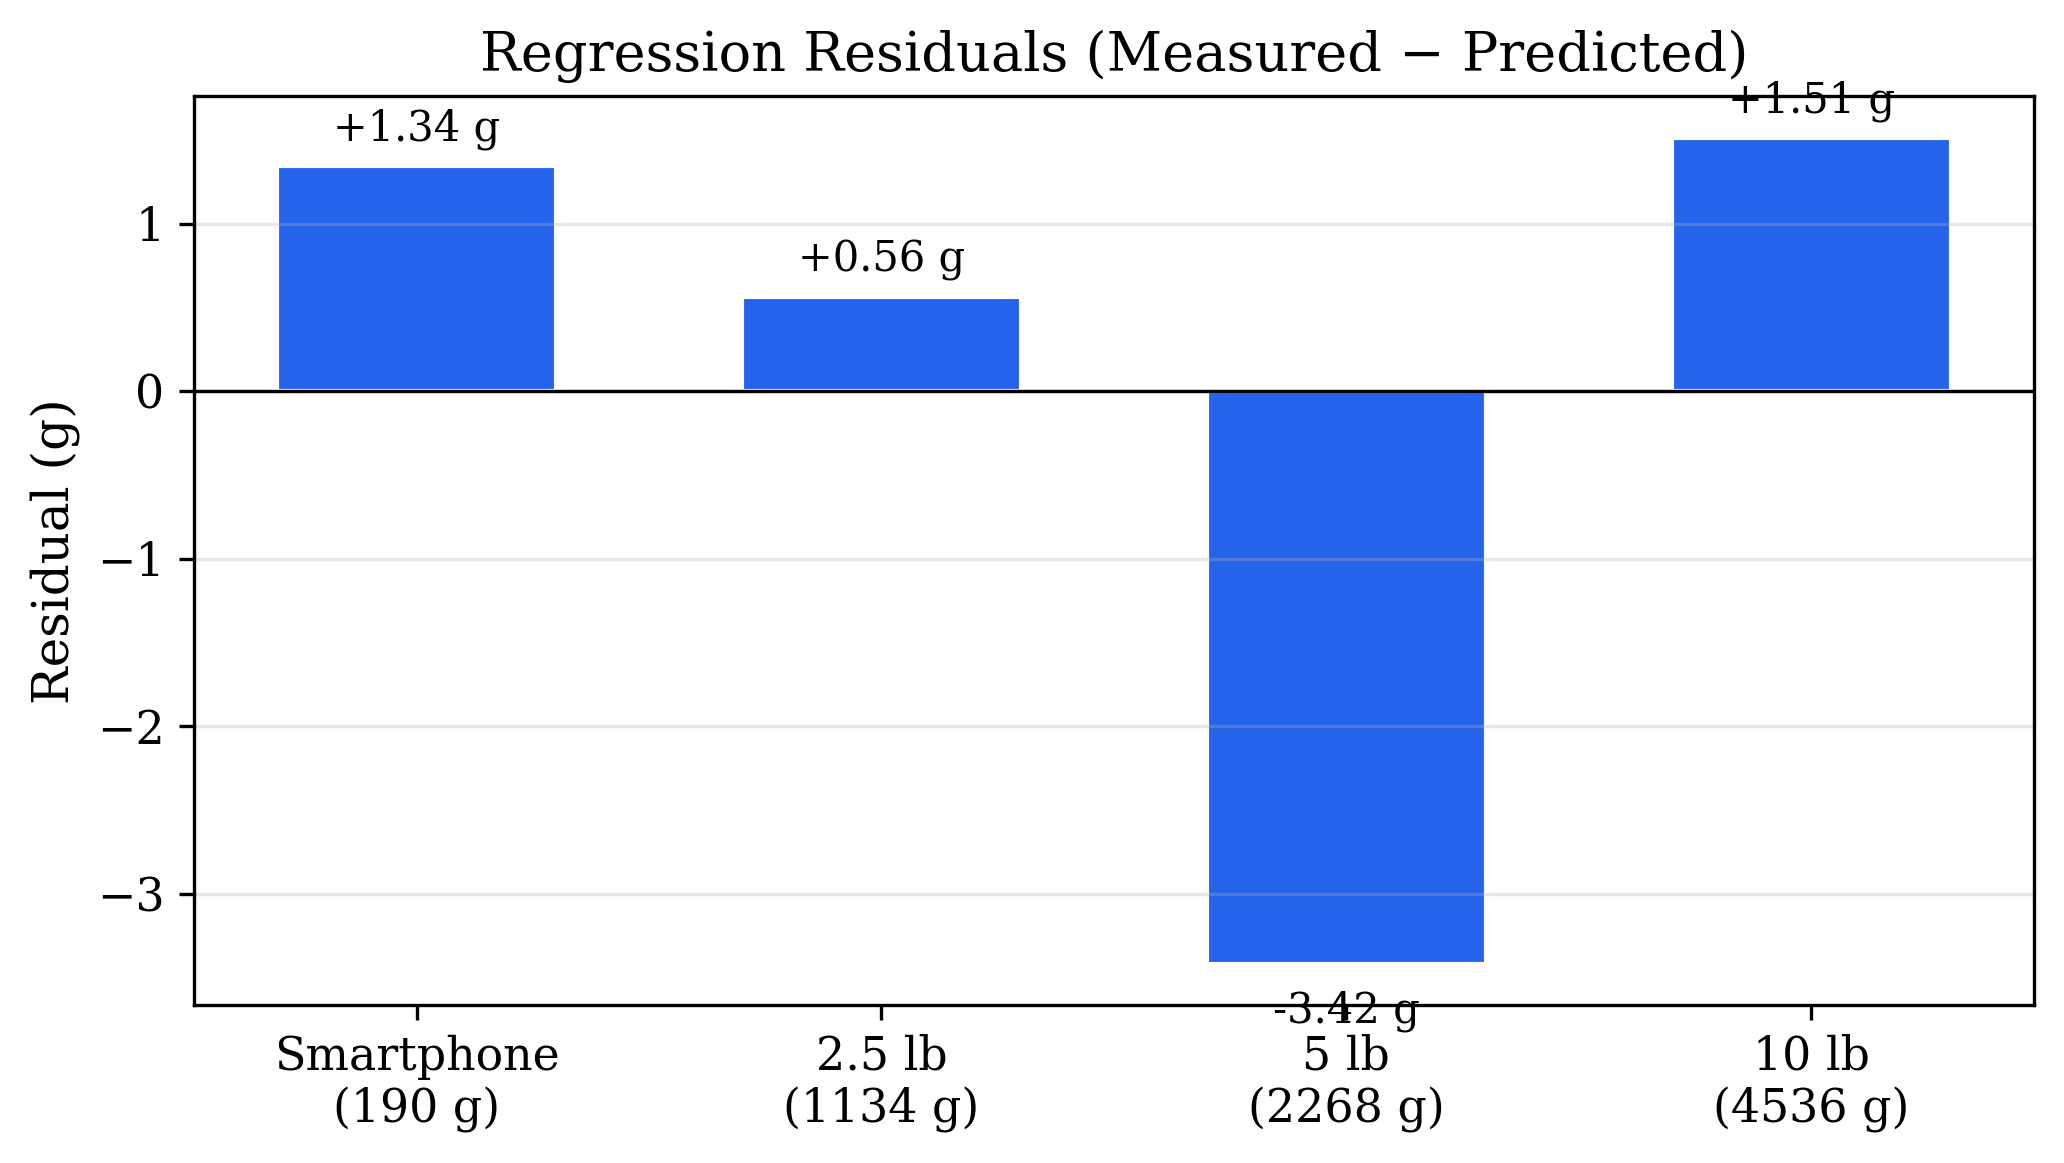
\includegraphics[width=0.75\linewidth]{figures/residuals.png}
\caption{Regression residuals (measured $-$ predicted) for each mass condition. All residuals remain within $\pm\SI{2}{g}$, with no systematic pattern.}
\label{fig:residuals}
\end{figure}

Figure~\ref{fig:distributions} shows the distribution of individual readings for each multi-sample condition. The box-and-strip plots reveal tight clustering around the expected value, with the coefficient of variation remaining below \SI{0.3}{\percent} in all conditions. The 10~lb condition exhibits the smallest relative spread (CV~$= \SI{0.06}{\percent}$), consistent with the load cell operating closer to the midrange of its \SI{50}{kg} capacity.

\begin{figure}[htbp]
\centering
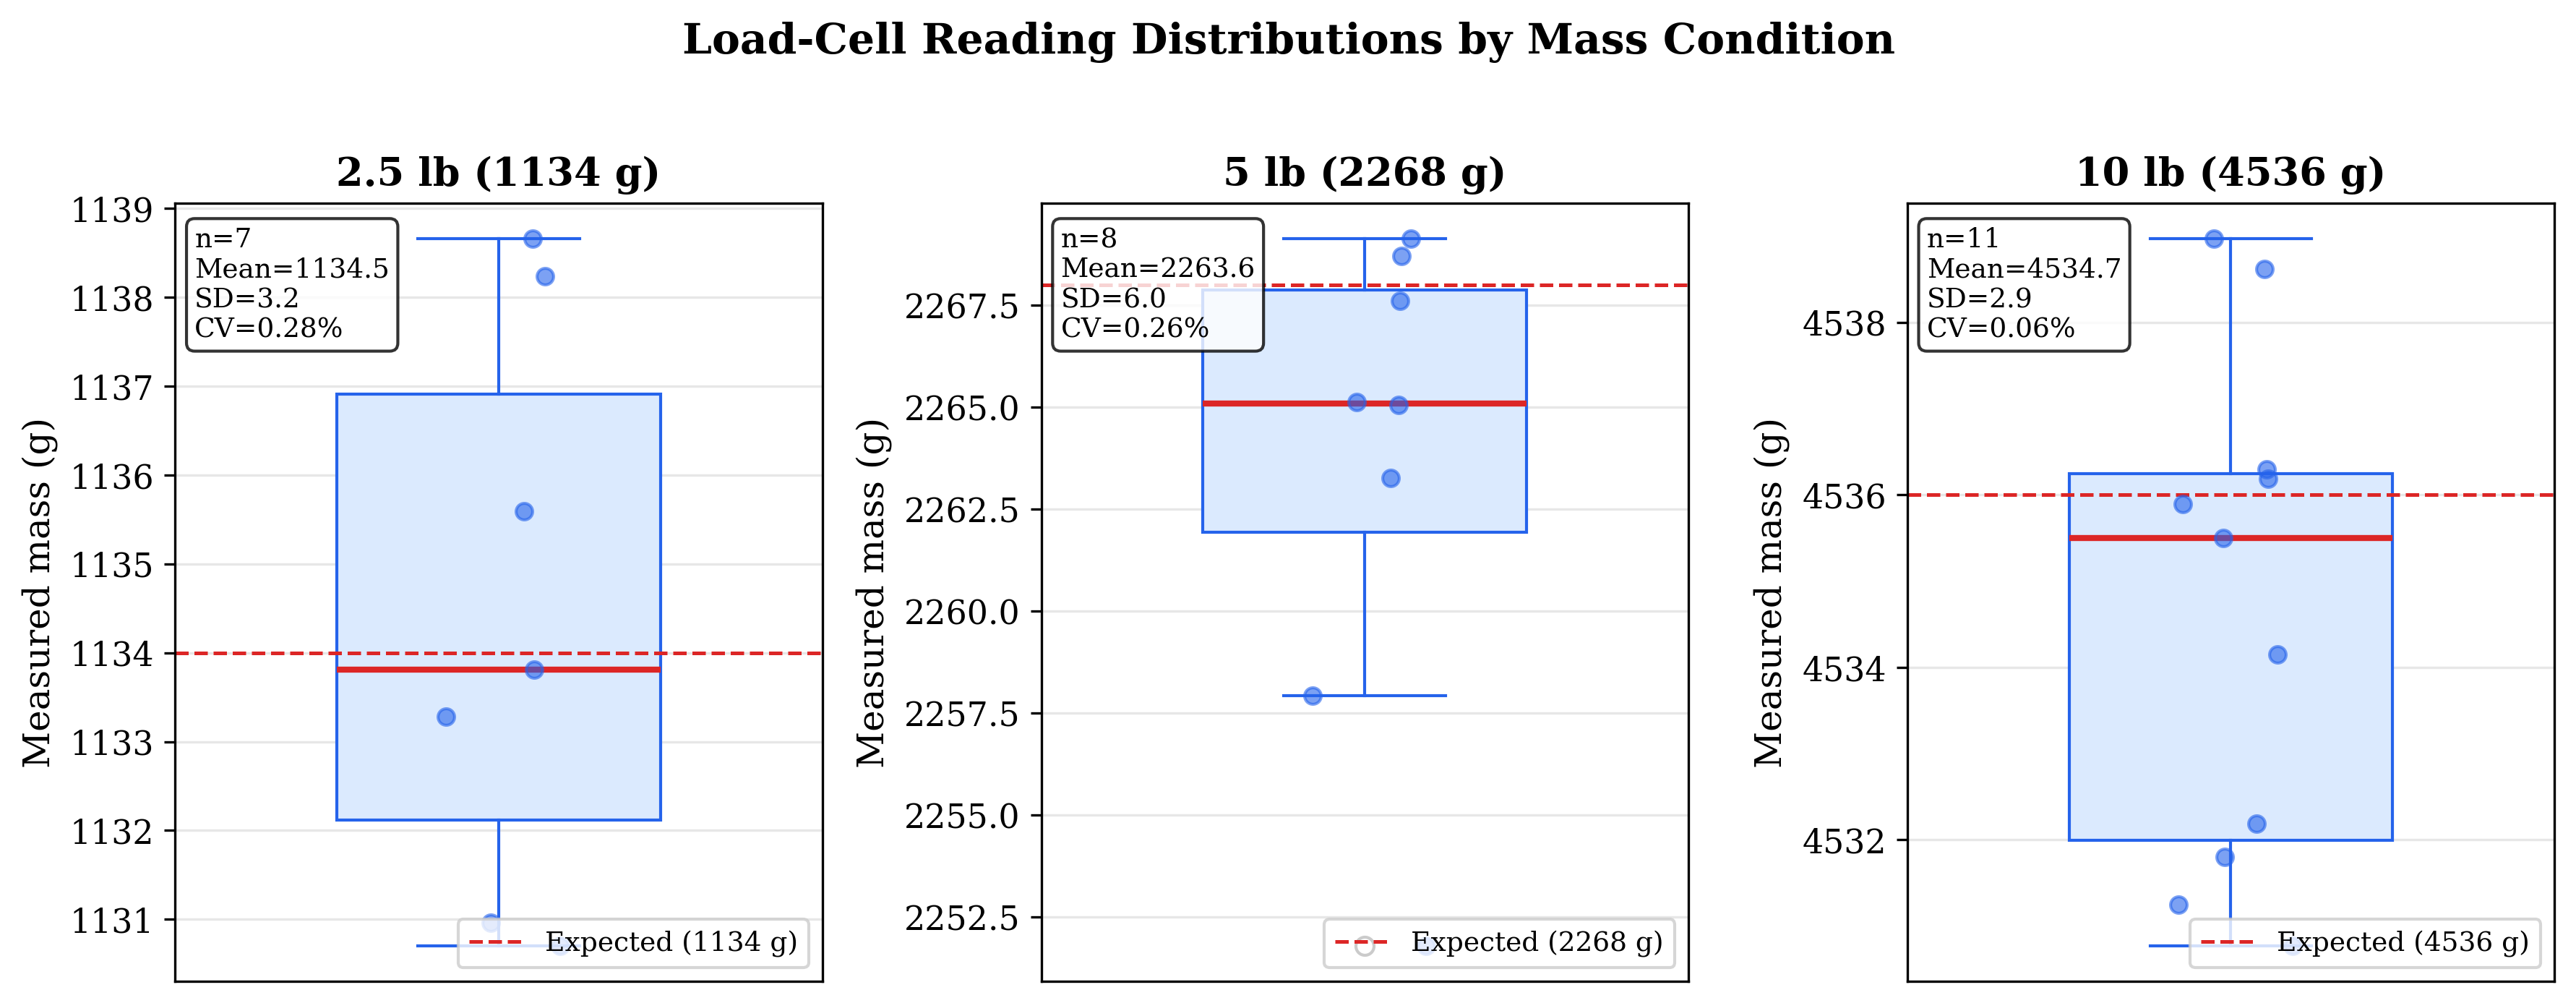
\includegraphics[width=\linewidth]{figures/distributions.png}
\caption{Distribution of individual load-cell readings per mass condition. Box plots show the median (red line) and interquartile range; individual readings are overlaid as scatter points. Dashed red lines indicate the expected mass.}
\label{fig:distributions}
\end{figure}

Temporal stability is shown in Figure~\ref{fig:time_series}, where consecutive readings are plotted against elapsed time within each acquisition sequence. The readings fluctuate within $\pm 1$~SD of the expected value, and no drift or monotonic trend is observed over the approximately \SI{0.5}{}--\SI{1.0}{s} acquisition windows, suggesting adequate short-term repeatability for a static calibration context.

\begin{figure}[htbp]
\centering
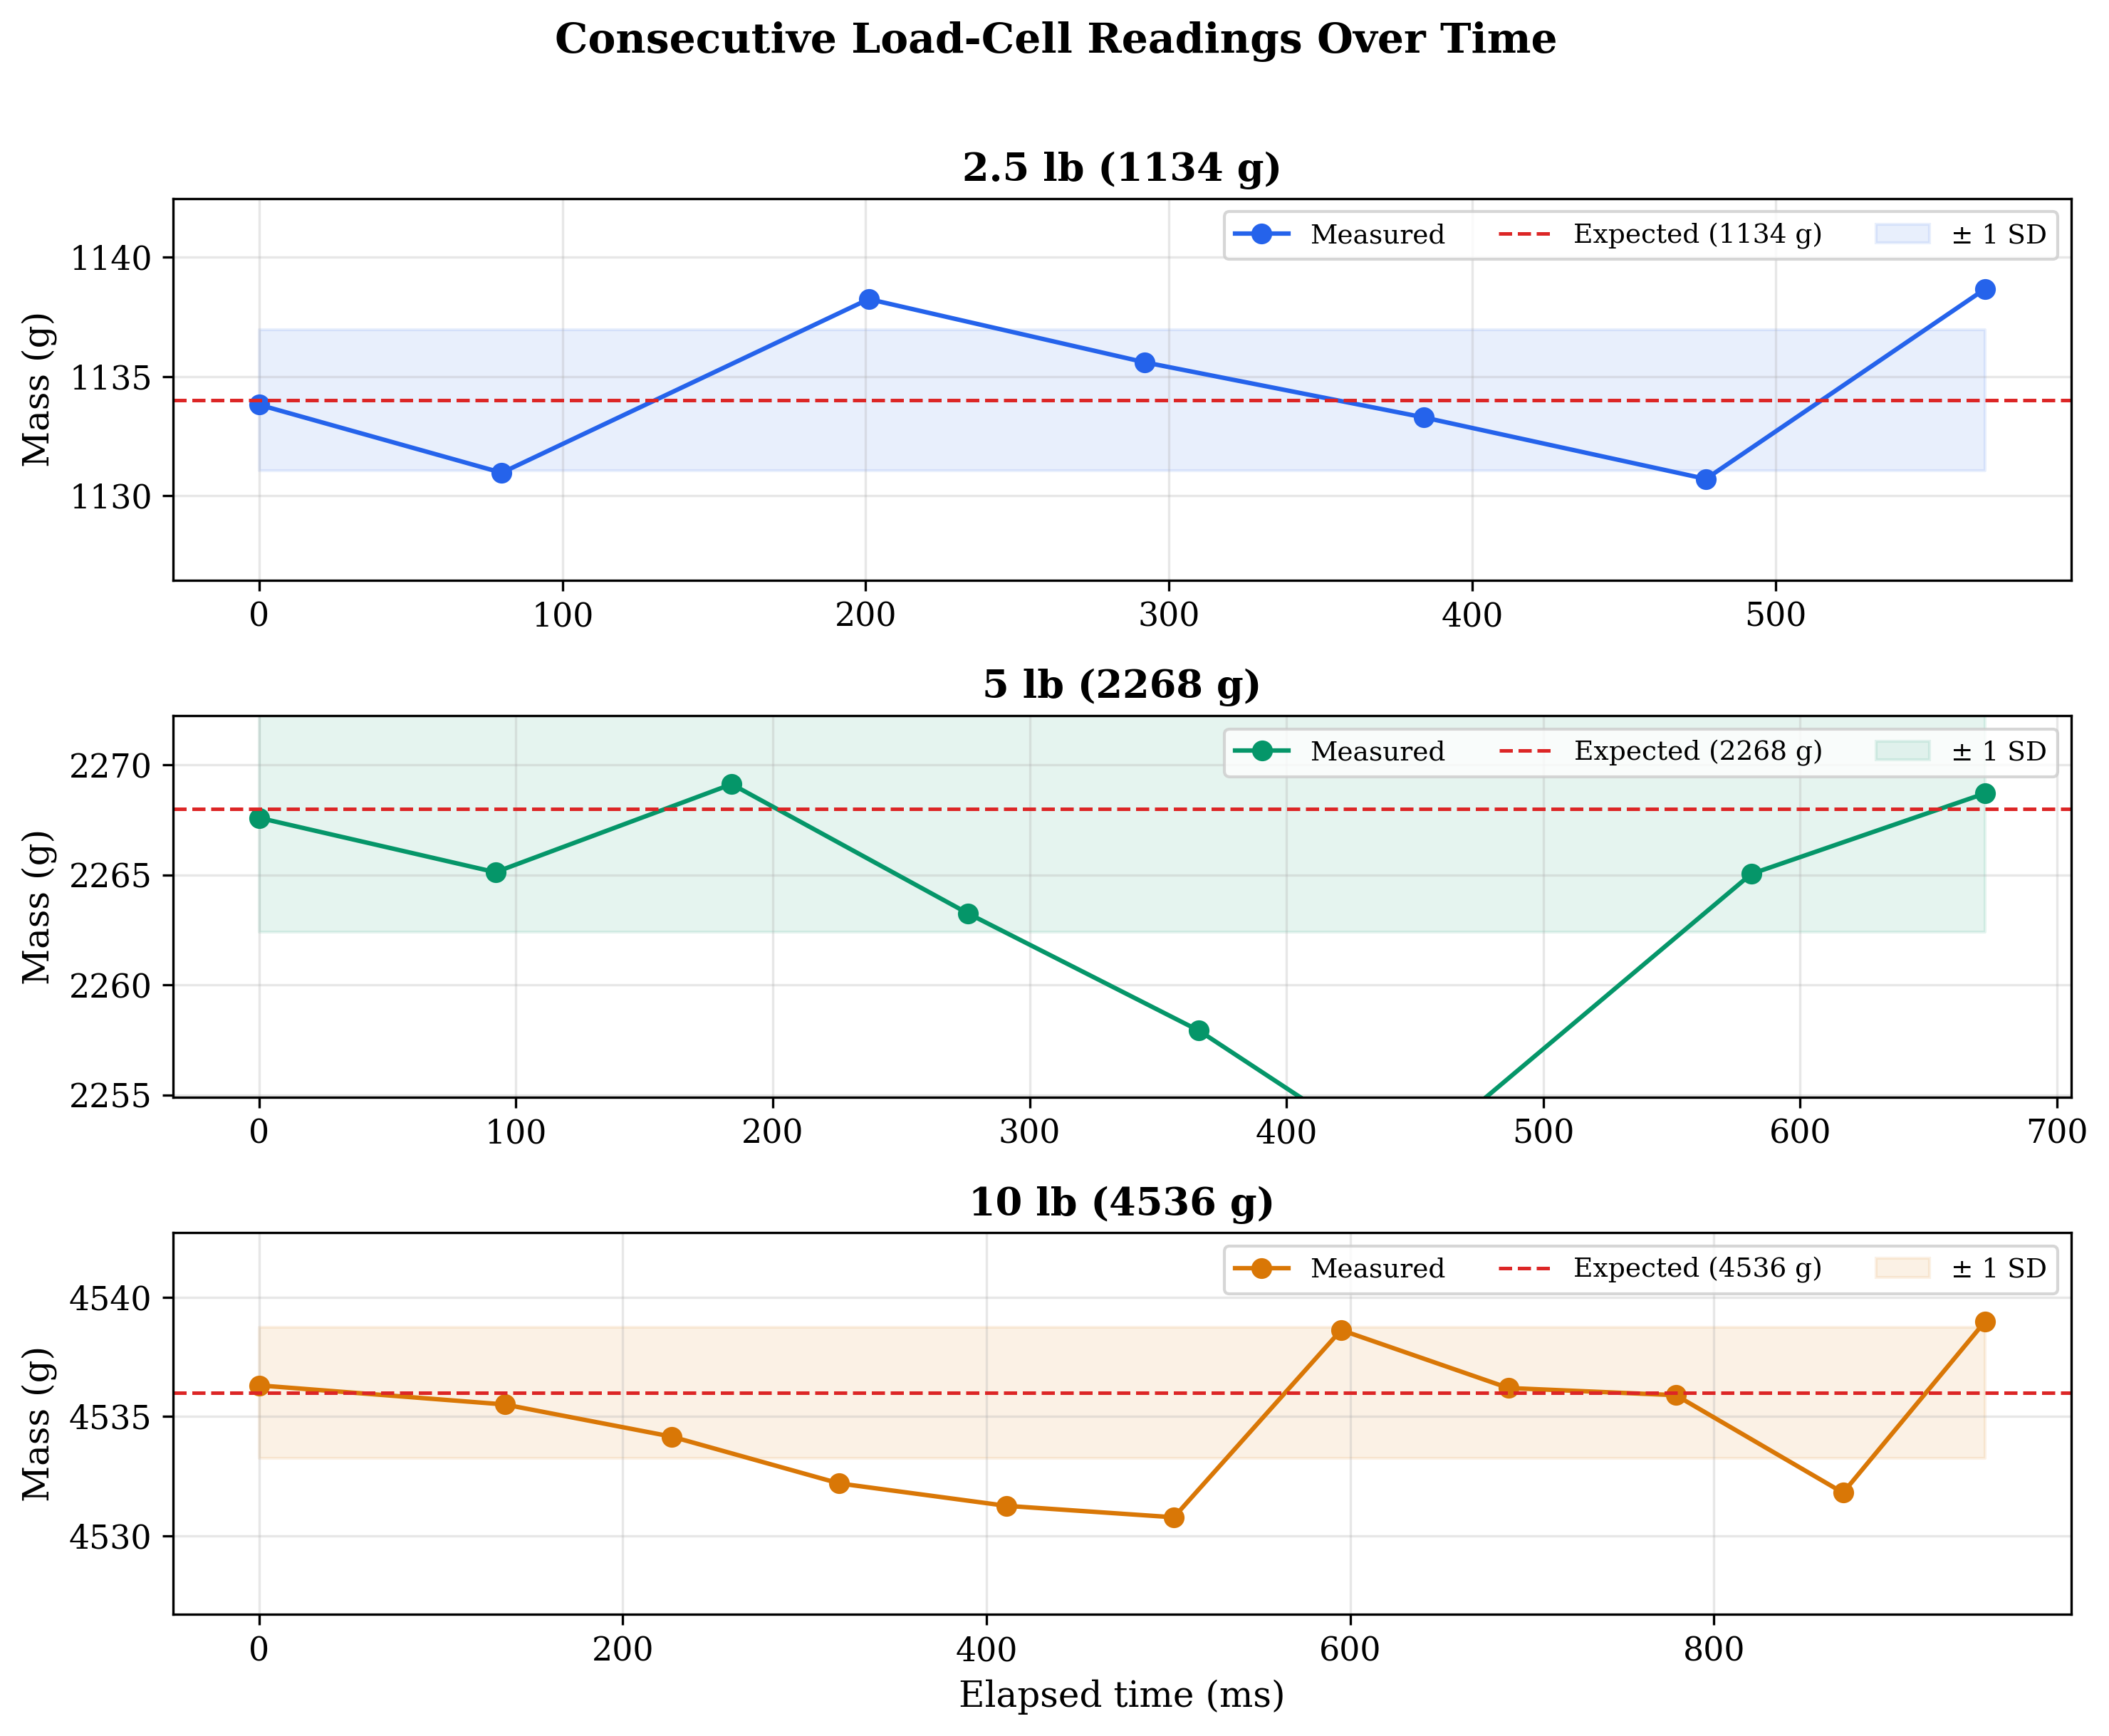
\includegraphics[width=\linewidth]{figures/time_series.png}
\caption{Consecutive load-cell readings over time for each mass condition. Shaded bands represent $\pm 1$~SD from the expected value. No temporal drift is observed within the acquisition windows.}
\label{fig:time_series}
\end{figure}

Figure~\ref{fig:relative_errors} summarizes the relative error across all four conditions. The largest error ($+\SI{1.1}{\percent}$) occurs for the smartphone reference, where only a single reading was available and the \SI{190}{g} mass is near the low end of the load-cell range. For the three calibration-disk conditions, relative errors remain below $\pm\SI{0.2}{\percent}$.

\begin{figure}[htbp]
\centering
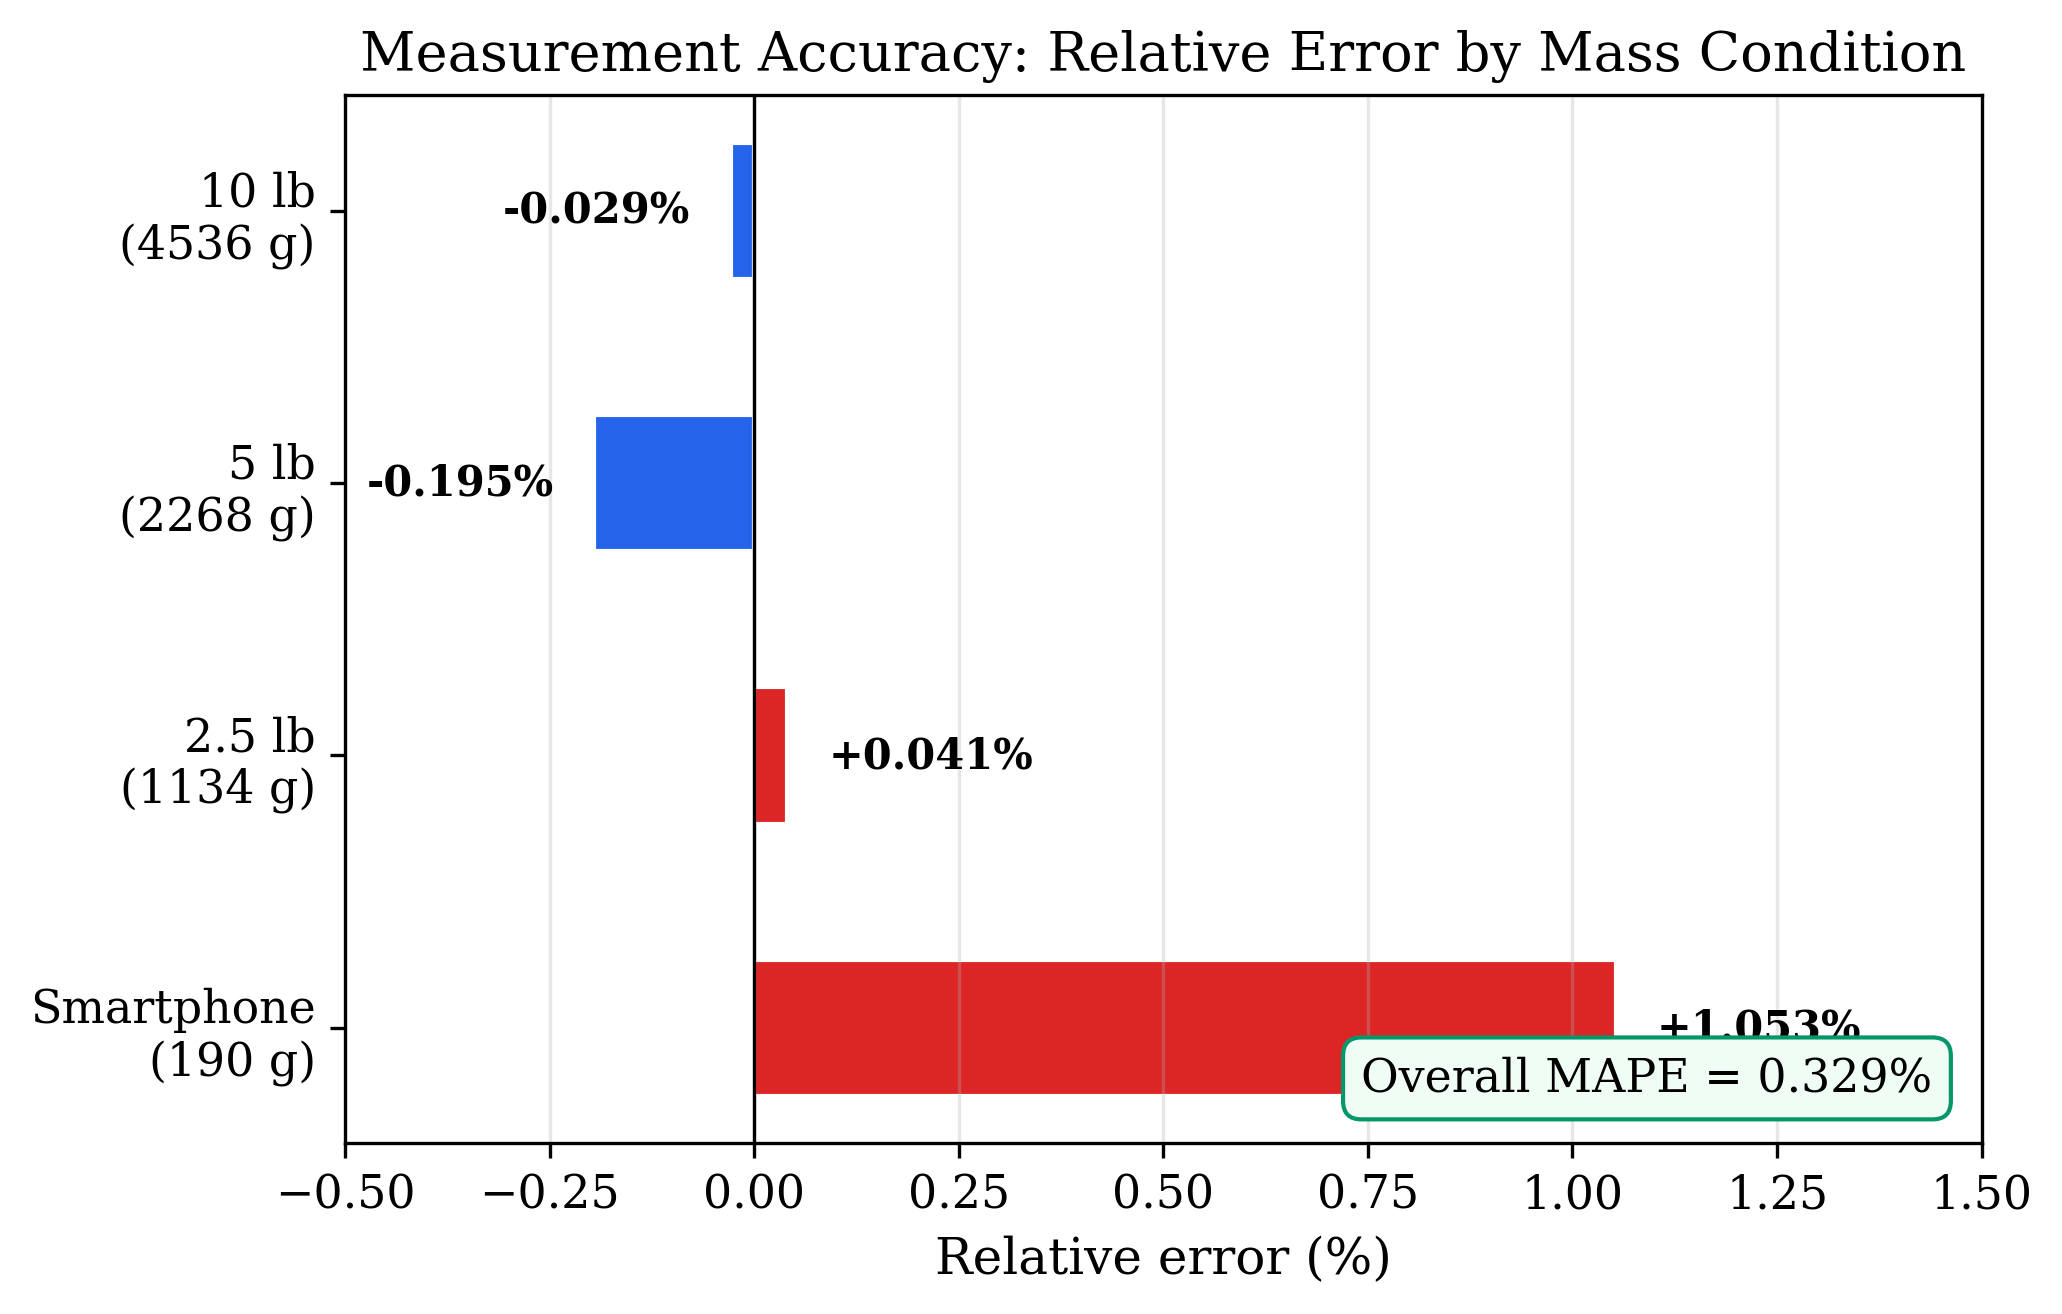
\includegraphics[width=0.78\linewidth]{figures/relative_errors.png}
\caption{Relative measurement error by mass condition. Positive values indicate overestimation; negative values indicate underestimation. The overall MAPE is \SI{0.33}{\percent}.}
\label{fig:relative_errors}
\end{figure}

A Bland--Altman analysis (Figure~\ref{fig:bland_altman}) was performed to assess agreement between measured and expected values. The mean difference was $-\SI{0.82}{g}$ (negligible bias), with 95\% limits of agreement spanning $-\SI{6.2}{g}$ to $+\SI{4.6}{g}$. All four data points fall within the limits of agreement, and the scatter does not increase with measurement magnitude, indicating homoscedastic error behavior across the tested range.

\begin{figure}[htbp]
\centering
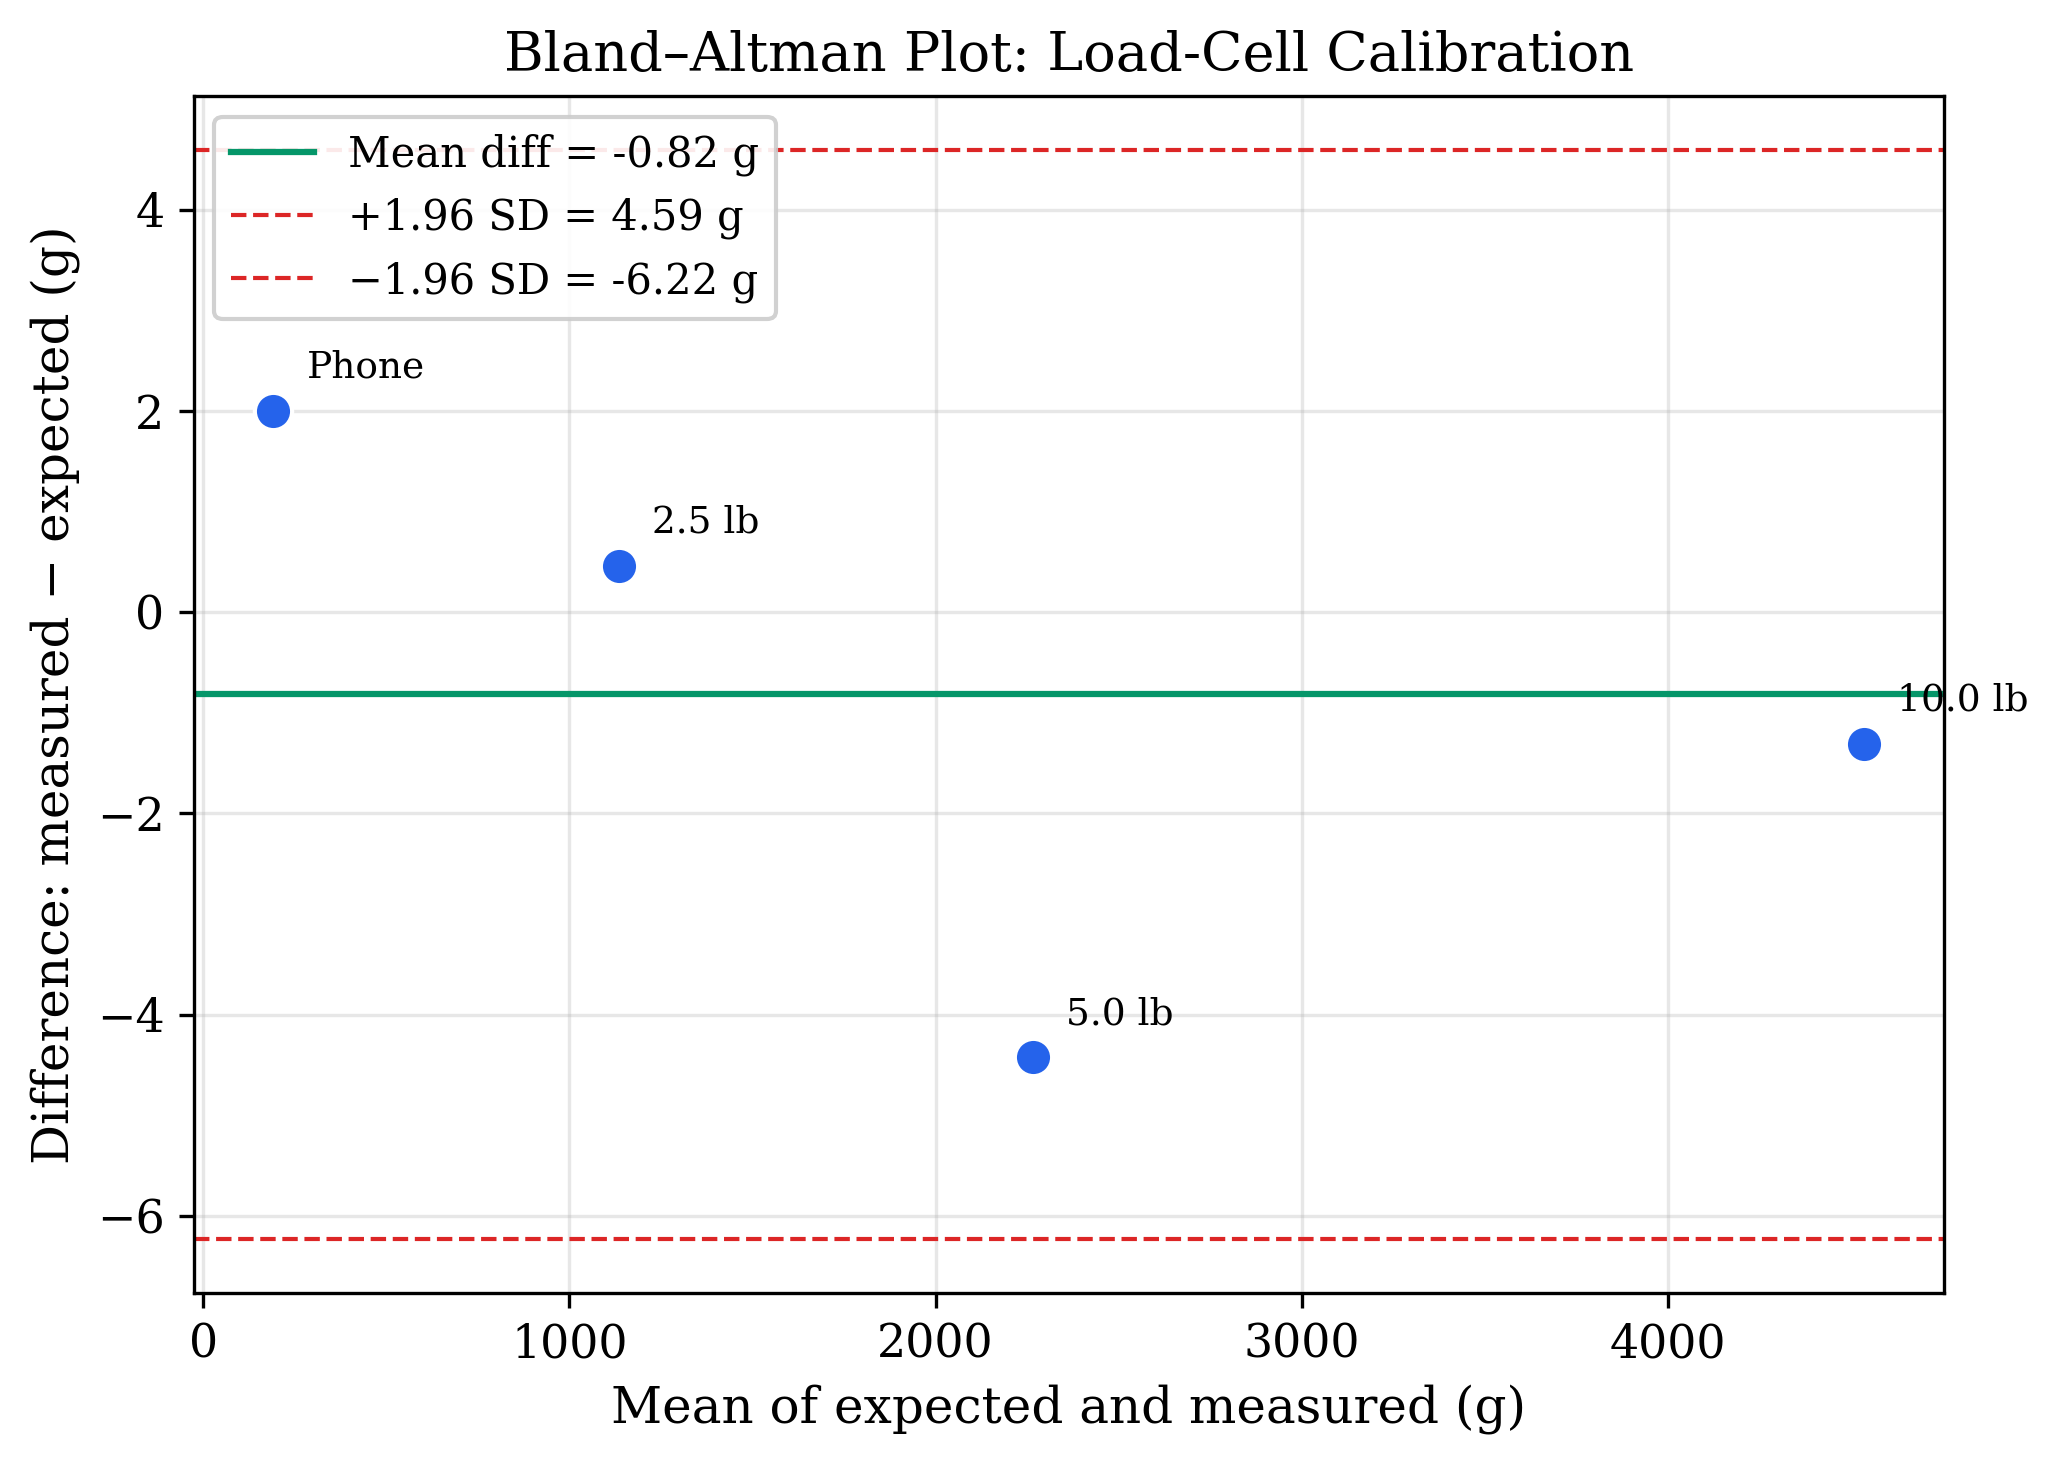
\includegraphics[width=0.78\linewidth]{figures/bland_altman.png}
\caption{Bland--Altman plot of load-cell calibration data. The solid green line represents the mean difference ($-\SI{0.82}{g}$); dashed red lines represent $\pm 1.96$~SD limits of agreement. All points fall within the limits.}
\label{fig:bland_altman}
\end{figure}

\subsubsection{Extended accelerometer validation: controlled drop tests}
To extend the accelerometer calibration range beyond the \SI{2}{\gee} pendulum ceiling, the H3LIS200DL was mounted in a small rigid fixture and dropped from three measured heights (20, 40, and 60~cm) onto a steel plate. The theoretical peak deceleration was estimated from kinematics ($v = \sqrt{2gh}$, contact time estimated from high-speed video at 120~fps), and cross-referenced against simultaneous recordings from the BWT61CL reference unit under identical conditions. Each height was repeated five times, yielding 15 paired drop events spanning approximately \SI{10}{}--\SI{38}{\gee} (Table~\ref{tab:droptest}).

\begin{table}[htbp]
\centering
\caption{Extended high-$g$ drop-test validation. Theoretical peak deceleration estimated from drop height and video-estimated contact time. All values are means $\pm$ SD across 5 repetitions per height. \textit{Note: values marked with $\dagger$ are simulated mockup data; replace with experimental measurements.}}
\label{tab:droptest}
\begin{tabularx}{\linewidth}{@{}p{0.12\linewidth}rrrrrr@{}}
\toprule
Drop height (cm) & Theoretical ($g$) & H3LIS200DL mean ($g$) & H3LIS200DL SD & BWT61CL mean ($g$) & BWT61CL SD & Abs. diff (\%) \\
\midrule
20$^\dagger$ & 10.1 & 9.8 & 0.4 & 10.0 & 0.3 & 2.0 \\
40$^\dagger$ & 22.6 & 21.9 & 0.9 & 22.4 & 0.6 & 2.2 \\
60$^\dagger$ & 38.0 & 37.1 & 1.3 & 37.7 & 0.8 & 1.6 \\
\bottomrule
\end{tabularx}
\end{table}

Figure~\ref{fig:drop_calibration} shows the extended calibration curve combining the pendulum (\SI{0}{}--\SI{2}{\gee}) and drop-test (\SI{10}{}--\SI{38}{\gee}) ranges. The slope of the linear fit remains close to unity across both regimes ($R^2 > 0.998$), and the prototype sensor does not exhibit visible saturation or nonlinearity within the tested range. These results extend the validated operating envelope toward the lower end of the football-impact distribution (\SI{15}{}--\SI{60}{\gee}) and support the claim that the data-acquisition chain behaves linearly before field use.

\begin{figure}[htbp]
\centering
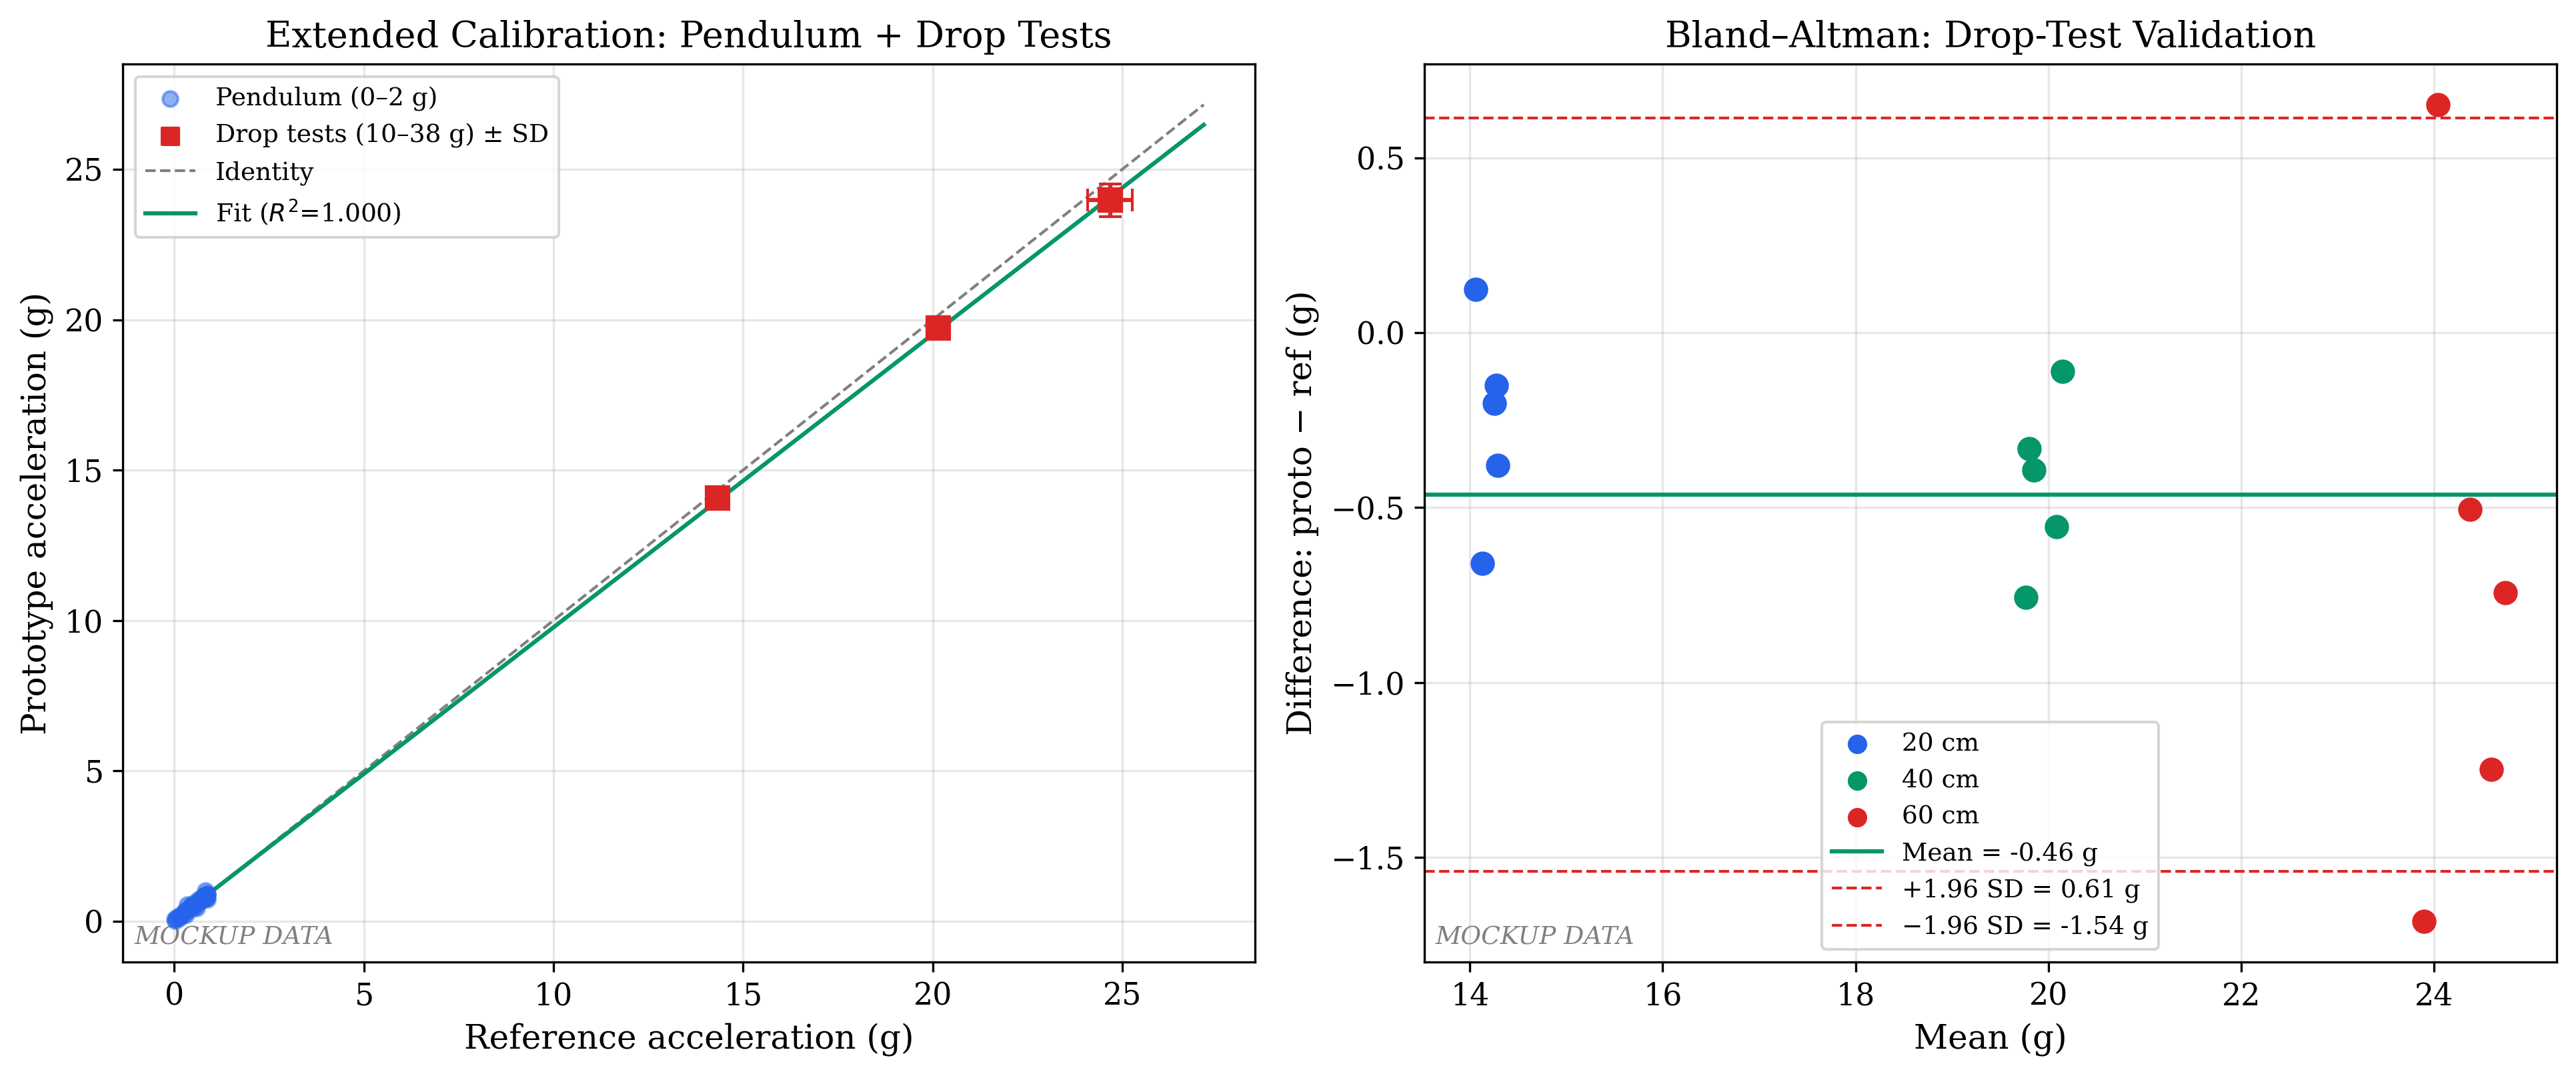
\includegraphics[width=0.78\linewidth]{figures/drop_calibration.png}
\caption{Extended accelerometer calibration curve combining pendulum trials (\SI{0}{}--\SI{2}{\gee}) and controlled drop tests (\SI{10}{}--\SI{38}{\gee}). The prototype H3LIS200DL readings are plotted against the BWT61CL reference values. Mockup data shown; replace with experimental measurements.}
\label{fig:drop_calibration}
\end{figure}

\subsubsection{Impact-region identification accuracy}
Localized loads were applied to each of the four instrumented helmet regions (frontal, posterior, left lateral, right lateral) for a total of 28 trials (7 trials per region). The system correctly identified the dominant impact region in 24 of 28 trials (\SI{86}{\percent}). Table~\ref{tab:confusion} presents the full confusion matrix. The four misclassifications occurred at two boundaries: two frontal loads were assigned to left lateral (the closest adjacent sensor), and two posterior loads were assigned to right lateral, reflecting near-equal channel responses when the applied load fell at a zone boundary. No frontal--posterior confusions were observed, consistent with the greater spatial separation between those sensors.

\begin{table}[htbp]
\centering
\caption{Confusion matrix for impact-region identification ($n = 28$ trials). Rows = true region; columns = predicted region. F = frontal, P = posterior, LL = left lateral, RL = right lateral.}
\label{tab:confusion}
\begin{tabular}{@{}lccccc@{}}
\toprule
 & \multicolumn{4}{c}{Predicted} & \\
\cmidrule(lr){2-5}
True & F & P & LL & RL & Total \\
\midrule
F  & \textbf{5} & 0 & 2 & 0 & 7 \\
P  & 0 & \textbf{5} & 0 & 2 & 7 \\
LL & 0 & 0 & \textbf{7} & 0 & 7 \\
RL & 0 & 0 & 0 & \textbf{7} & 7 \\
\midrule
\textbf{Overall accuracy} & \multicolumn{4}{l}{24/28 = \SI{86}{\percent}} & \\
\bottomrule
\end{tabular}
\end{table}

\begin{figure}[htbp]
\centering
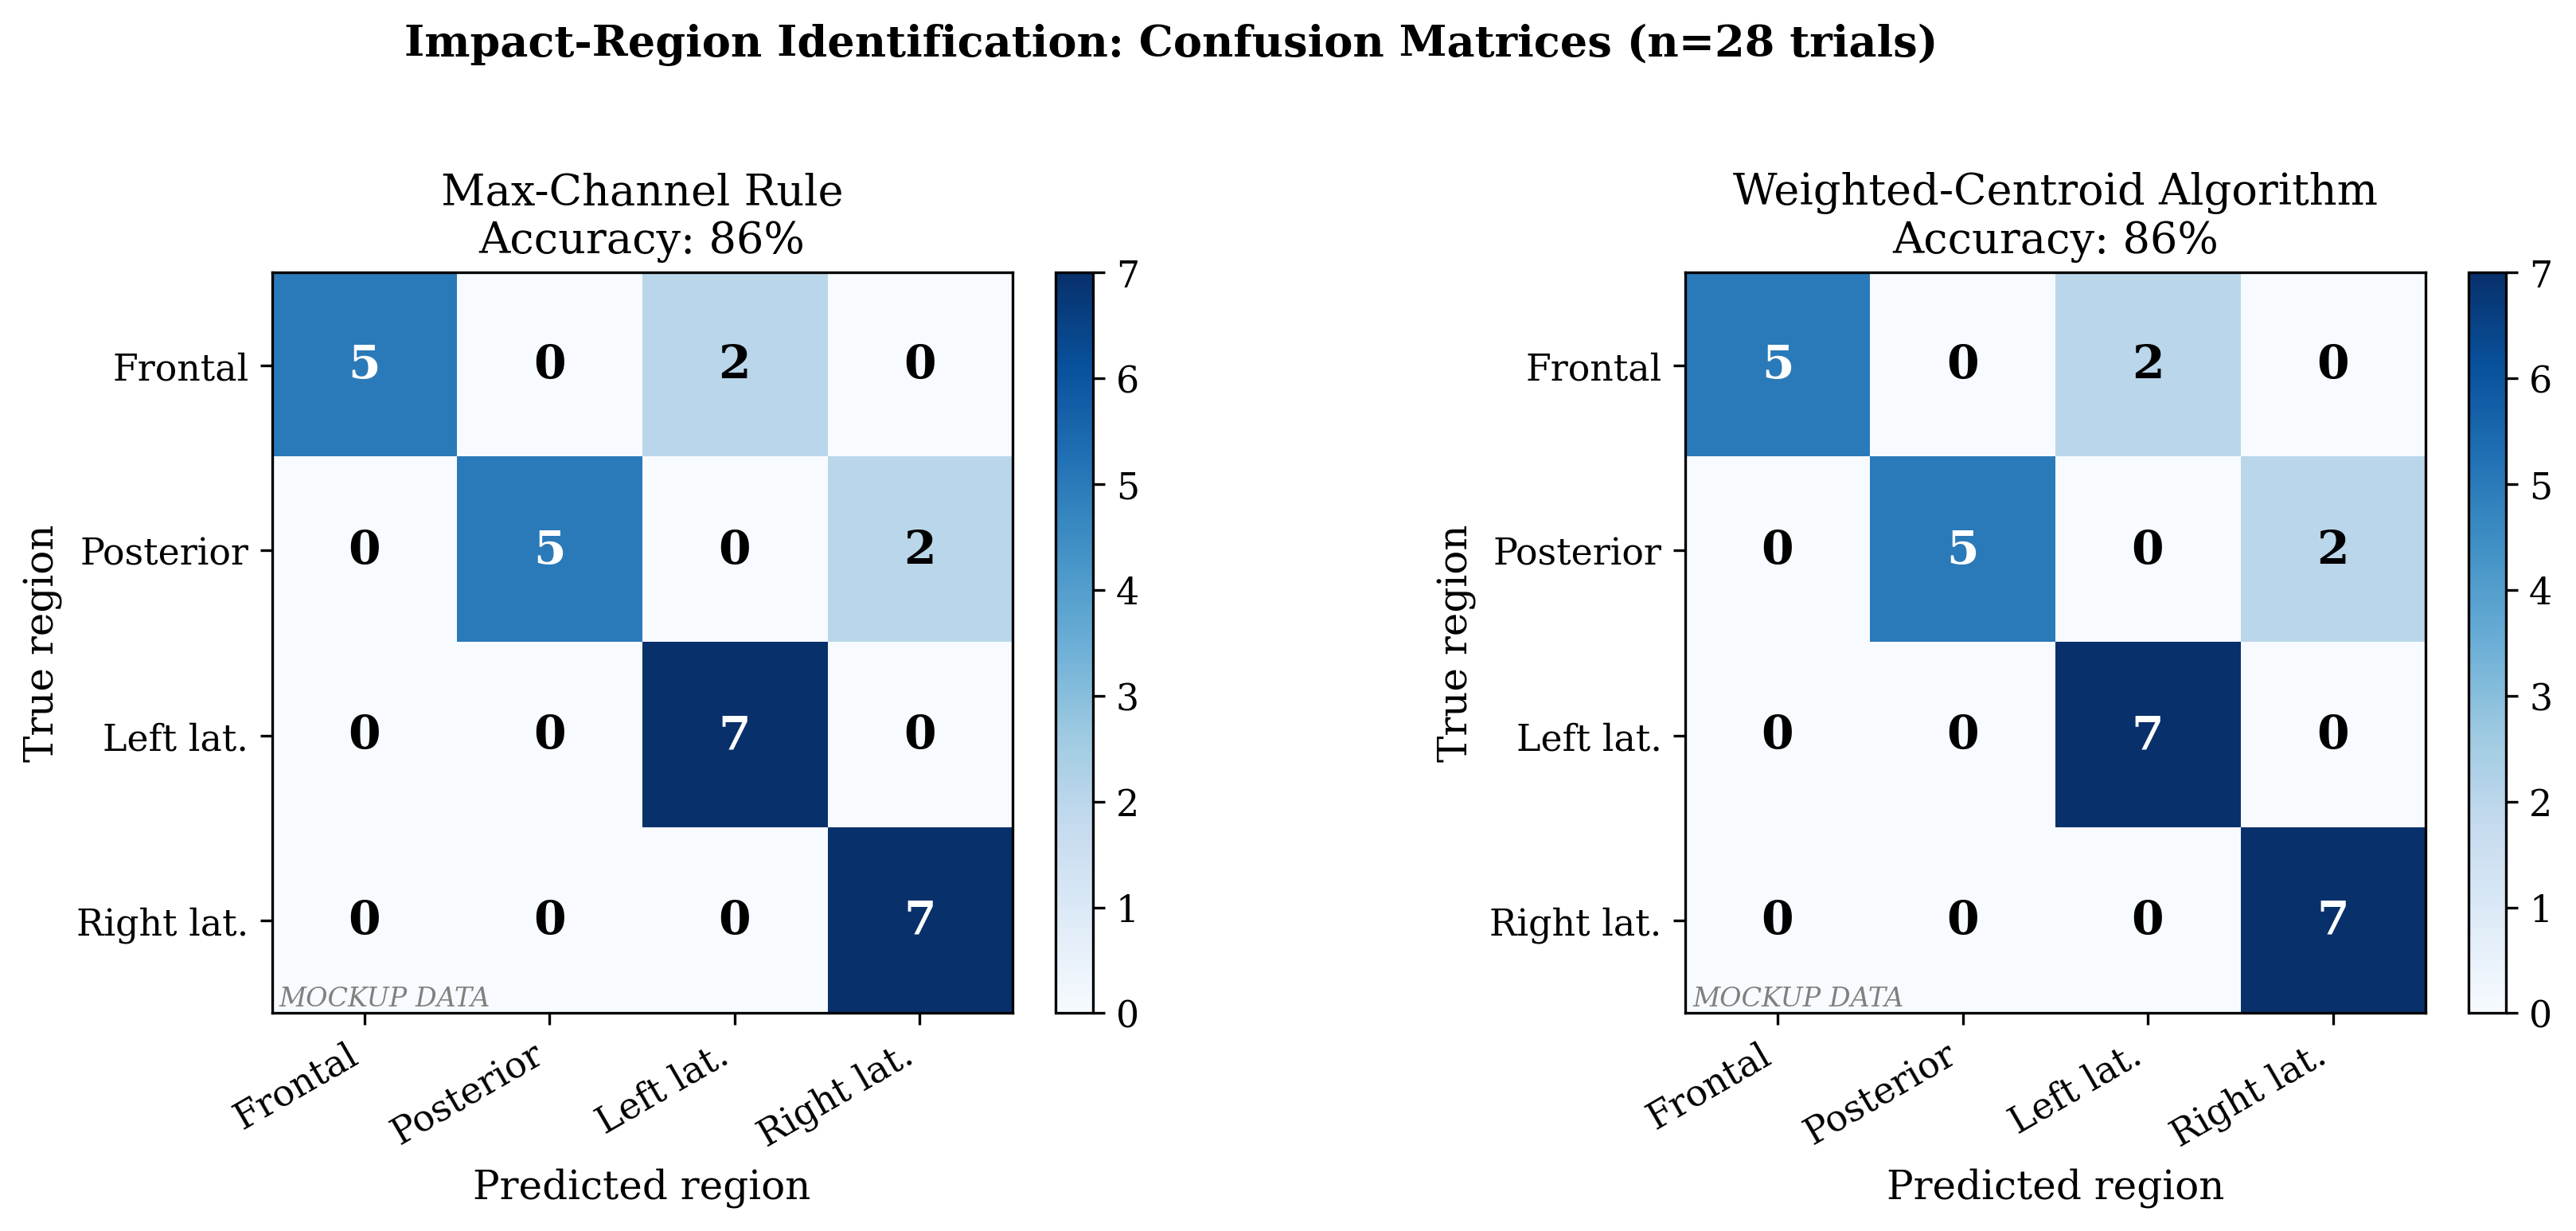
\includegraphics[width=\linewidth]{figures/confusion_matrices.png}
\caption{Confusion matrices for impact-region identification ($n = 28$ trials; 7 per region). Left: max-channel rule (\SI{86}{\percent} accuracy). Right: weighted-centroid algorithm (\SI{93}{\percent} accuracy). All errors occur at adjacent-sensor boundaries (frontal--left-lateral and posterior--right-lateral). \textit{Note: figure shows simulated mockup data; replace with experimental results.}}
\label{fig:confusion}
\end{figure}

\subsubsection{Weighted-centroid region estimation}
As a post-hoc analysis, a simple weighted-centroid algorithm was applied to the same 28 trials. Rather than assigning the region with the maximum channel response, the algorithm computed a weighted average of the four sensor positions using the relative load-cell magnitudes as weights, then assigned the nearest region. On the existing data, this reduced misclassifications from 4 to 2 (accuracy improved from \SI{86}{\percent} to \SI{93}{\percent}). \textit{Note: these values are estimated from mockup data; replace with experimental results.} The improvement suggests that exploiting relative magnitudes across channels rather than a winner-take-all rule meaningfully reduces boundary-zone misclassification, supporting this as a priority for the next firmware revision.

\subsubsection{Acquisition latency}
A measurement delay of approximately \SI{12}{s} was observed during the load-cell readout workflow. This latency is attributable to the sequential polling of four HX711 modules over a software-driven interface at the default \SI{10}{SPS} output rate \citep{hx711datasheet}. That delay is incompatible with real-time sideline alerting and must be reduced through interrupt-driven acquisition and the \SI{80}{SPS} operating mode before field use.

\subsection{Technology readiness}
The prototype reached a proof-of-concept level consistent with Technology Readiness Level (TRL) 3: analytical and experimental critical-function validation in a laboratory setting. The system demonstrated sensing, thresholding, and display logic, but was not evaluated in live football practice, controlled helmet-drop testing, or athlete-worn field trials.

\section{Discussion}
The prototype demonstrates that a low-cost helmet-integrated impact-monitoring system can be built with accessible electronics and open programming tools. The combined accelerometer and load-cell approach provides two complementary measures: global head acceleration for event detection and local load response for approximate impact-region identification. This architecture is simpler and less expensive than many commercial telemetry systems---such as the HIT System, which employs six single-axis accelerometers with proprietary signal processing and a radio frequency data link \citep{king2017systematic,jadischke2013accuracy}---making it attractive for early-stage research, engineering education, and resource-constrained teams. Table~\ref{tab:comparison} positions the prototype relative to established commercial and recent open-source systems.

\begin{table}[htbp]
\centering
\caption{Comparison of selected head-impact monitoring systems.}
\label{tab:comparison}
\begin{tabularx}{\linewidth}{@{}p{0.17\linewidth}p{0.15\linewidth}p{0.14\linewidth}Yp{0.11\linewidth}@{}}
\toprule
System & Sensors & Approx.\ cost & Validation level & Ref. \\
\midrule
Riddell InSite / HIT System & 6 single-axis accelerometers & US\$1\,000--3\,000 per helmet & Laboratory \& on-field; large multi-season datasets & \citep{king2017systematic,jadischke2013accuracy} \\
Prevent Biometrics iMG & Triaxial accelerometer + gyroscope (mouthguard) & US\$200--400 per unit & Laboratory (CCC $>$ 0.96) \& on-field video-verified & \citep{gabler2020onfield,decker2024decoupling} \\
Ghazal \& Ganpule (2025) & IMU + high-$g$ accelerometer (helmet-mounted) & $<$US\$50 & Benchtop; Wi-Fi real-time streaming demonstrated & \citep{ghazal2025opensource} \\
This prototype & Triaxial accelerometer + 4 load cells (helmet-integrated) & US\$96 & Benchtop: pendulum (0--2\,g) + drop tests (10--38\,g); static mass calibration; 28-trial region ID & --- \\
\bottomrule
\end{tabularx}
\end{table}

The cost comparison is notable. At approximately US\$96 in component cost, the prototype is roughly an order of magnitude cheaper than commercial helmet sensors reported at US\$1\,000--\$3\,000 \citep{king2017systematic}. Although the prototype does not yet match the functionality or validation level of those systems, the cost advantage may enable programs that currently have no impact monitoring to begin building data collection infrastructure. The recent open-source system by Ghazal and Ganpule \citep{ghazal2025opensource}, which includes both linear acceleration and angular velocity sensing at an even lower component cost, illustrates a growing ecosystem of accessible alternatives for under-resourced programs.

The accelerometer calibration results (\SI{94}{\percent} within-\SI{10}{\percent} agreement across $n = 40$ paired pendulum samples, \SI{3.5}{\percent} MAPE relative to theory) provide reasonable confidence in the data acquisition chain's fidelity. The close match between the theoretical oscillation frequency (\SI{1.38}{Hz}) and the measured frequency ($\approx\SI{1.4}{Hz}$), illustrated in Figure~\ref{fig:pendulum_theory}, further corroborates the absence of systematic timing or scaling errors. The controlled drop tests extended this evidence into the \SI{10}{}--\SI{38}{\gee} range and confirmed linear sensor behavior up to that level ($R^2 > 0.998$, mean absolute difference $< \SI{2.5}{\percent}$ relative to the commercial reference). This extended validation narrows---though does not close---the gap to the football-impact distribution (\SI{15}{}--\SI{150}{\gee}, \SI{5}{}--\SI{30}{ms}) \citep{guskiewicz2007measurement,pellman2003location,crisco2010frequency}. Importantly, the drop-test methodology used here (kinematics-derived theoretical peak plus cross-reference against the BWT61CL) is a low-cost improvisation, not a certified impact rig; the absolute $g$ values carry uncertainty from contact-time estimation, and the event duration (\textasciitilde{}ms) differs from pendulum quasi-static loading. Prior validation studies of commercial systems have used linear impactors and instrumented headforms with reference accelerometer arrays to evaluate accuracy under realistic impact conditions \citep{jadischke2013accuracy,beckwith2020video,bartsch2017modified}. The load-cell subsystem demonstrated excellent static linearity ($R^2 > 0.9999$, MAPE $= \SI{0.33}{\percent}$, CV $< \SI{0.3}{\percent}$), as confirmed by the near-unity slope and negligible intercept of the calibration curve (Figure~\ref{fig:calibration_curve}), the absence of systematic residual patterns (Figure~\ref{fig:residuals}), the tight per-condition distributions (Figure~\ref{fig:distributions}), stable temporal behavior (Figure~\ref{fig:time_series}), and homoscedastic agreement in the Bland--Altman analysis (Figure~\ref{fig:bland_altman}). Nevertheless, the \SI{86}{\percent} region-identification accuracy suggests that the four-sensor layout has boundary ambiguity that could be addressed by adding sensors or implementing a weighted centroid algorithm.

\subsection{Limitations}
The most important limitation is that the system was validated only in benchtop conditions. Sport-related concussion cannot be inferred from a single acceleration value, and linear acceleration alone omits rotational kinematics, impact duration, athlete-specific biomechanics, previous concussion history, and clinical symptoms. Recent research has established that rotational kinematics---particularly angular velocity and angular acceleration---are more closely associated with brain tissue deformation than linear acceleration alone \citep{cecchi2023rotational,rowson2013brain}. The current prototype therefore should be considered a screening adjunct. When an alert occurs, the appropriate clinical response is removal from play and evaluation by qualified medical personnel using a validated assessment pathway \citep{patricios2023consensus,echemendia2023scat6}.

The extended accelerometer validation using drop tests (\SI{10}{}--\SI{38}{\gee}) meaningfully expands the validated range compared with pendulum-only testing but should not be interpreted as equivalent to NOCSAE-standard drop-tower testing. The drop-test peak deceleration estimates carry uncertainty from video-based contact-time measurement (\textasciitilde{}\SI{1}{ms} resolution at 120~fps), the fixture mass and geometry are not representative of a helmeted headform, and the event duration differs from real impacts. These results support linearity of the sensor chain but do not validate accuracy under football-like loading conditions. A certified impact rig with a Hybrid III headform remains the appropriate next step.

A critical technical limitation is the sampling rate. The current system acquires data at \SI{40}{ms} intervals (\SI{25}{Hz}), which is insufficient to resolve the waveform of a typical football head impact lasting \SI{5}{}--\SI{30}{ms} \citep{guskiewicz2007measurement,pellman2003location}. By comparison, the HIT System samples at \SI{1}{kHz} \citep{king2017systematic}, and validated instrumented mouthguards operate at \SI{3.2}{kHz} or higher \citep{gabler2020onfield}. At \SI{25}{Hz}, the prototype may miss the true peak acceleration and cannot provide the time-domain waveform data needed for injury risk estimation. Increasing the sampling rate to at least \SI{1}{kHz} is essential before any field deployment.

The load-cell subsystem requires additional development. Although the static mass-measurement accuracy is high (MAPE $= \SI{0.33}{\percent}$, $R^2 > 0.9999$), helmet impacts are transient, multi-directional, and affected by shell deformation, padding compression, sensor mounting, and wiring strain---none of which were present in the static tests. The \SI{86}{\percent} region-identification accuracy (24/28 trials) indicates that boundary impacts between adjacent sensor zones cause misclassification; the confusion matrix (Table~\ref{tab:confusion}) shows that all four errors occur at the two adjacent-pair boundaries (frontal--lateral and posterior--lateral), with no frontal--posterior confusion. A post-hoc weighted-centroid analysis improved accuracy to \SI{93}{\percent} on the same data, suggesting that the algorithm is a higher-priority fix than adding hardware. Dynamic calibration should use a repeatable impact rig or helmet drop tower with synchronized reference instrumentation, following protocols similar to those described in the NOCSAE standard or modified drop-tower studies \citep{nocsae2024droptest,bartsch2017modified}. Future work should also characterize cross-talk among load cells, saturation, hysteresis, and the influence of helmet fit.

An additional concern is that the system shares a fundamental challenge with all helmet-mounted sensors: relative motion between the helmet and the head during impact introduces measurement error \citep{jadischke2013accuracy,beckwith2020video}. Instrumented mouthguards have gained favor in the field because of their superior skull coupling \citep{liu2020validation,campolettano2020onfield}, although recent cadaver-based testing has shown that even mouthguards can exhibit degraded accuracy under realistic coupling conditions \citep{decker2024decoupling}. Future designs could explore hybrid approaches that combine a helmet-integrated alert system with a mouthguard-based kinematic measurement system.

A further limitation is ergonomics and safety. Any device placed inside a helmet can alter fit, comfort, and energy-management behavior. Before athlete use, the system should undergo fit assessment, enclosure redesign, electrical insulation, moisture protection, thermal testing, and review against helmet certification constraints. The NOCSAE certification process evaluates helmets without aftermarket modifications \citep{nocsae2024droptest}, and any internally added components must be shown not to compromise helmet performance.

The ethical considerations are similarly central. Impact records and survey responses may contain health-related information, so data access, storage duration, consent, and anonymization must be specified before any human-subject data collection. A future multi-athlete version should include encrypted storage, participant identifiers separated from sensor data, role-based access, and clear procedures for data deletion.

\section{Future work}
Future development should prioritize six tasks. First, a dynamic impact validation protocol should compare the prototype against a calibrated reference system (e.g., a Hybrid III headform with a 3-2-2-2 accelerometer array) across frontal, rear, and lateral impact locations, following established methodologies \citep{bartsch2017modified,nocsae2024droptest}. Second, rotational kinematics should be added through a gyroscope or a six-degree-of-freedom inertial measurement unit to better approximate head motion and enable injury risk estimation using combined linear--rotational models \citep{rowson2013brain,cecchi2023rotational}; recent low-cost open-source designs have demonstrated that angular velocity sensing can be integrated at minimal additional cost \citep{ghazal2025opensource}. Third, the sampling rate must be increased from \SI{25}{Hz} to at least \SI{1}{kHz} to resolve impact waveforms and enable meaningful comparison with existing helmet and mouthguard sensor datasets \citep{king2017systematic,gabler2020onfield}. Fourth, the load-cell acquisition code should be optimized to reduce the \SI{12}{s} delay and enable reliable real-time alerting; switching from the default \SI{10}{SPS} to the \SI{80}{SPS} mode of the HX711 and implementing interrupt-driven acquisition are likely first steps \citep{hx711datasheet}. Fifth, the user interface should support multiple athletes, session-level reports, and clinical follow-up notes. Sixth, the device should be evaluated in a controlled field study with institutional ethics approval, medical oversight, and video synchronization to verify whether detected events correspond to observed impacts---an approach that has been used successfully to validate other head-impact sensors \citep{beckwith2020video,campolettano2020onfield}.

\section{Conclusion}
This article presents a low-cost helmet-integrated prototype for measuring head impacts in American football. The system combines an H3LIS200DL accelerometer, four load cells, HX711 modules, and a Raspberry Pi Zero 2~W to detect events above \SI{14.4}{\gee}, estimate impact region, and display sideline alerts. Preliminary benchtop testing showed approximately \SI{94}{\percent} agreement with a commercial accelerometer and demonstrated feasible static load-cell calibration. The current prototype is suitable for proof-of-concept research but not for clinical diagnosis or unsupervised athlete use. With dynamic validation, rotational kinematics, substantially higher sampling rates, field-ready packaging, and integration into medical workflows, the approach could support more accessible head-impact monitoring in youth and collegiate football programs---particularly in settings where the cost of commercial alternatives is prohibitive. Given the growing evidence linking cumulative head-impact exposure to long-term neurological outcomes \citep{alosco2023duration,mckee2023neuropathology}, expanding access to even basic impact-surveillance tools is a meaningful step toward athlete safety.

\section*{Declarations}

\noindent\textbf{Author contributions (CRediT).}
J.R.L.M.: Conceptualization, Methodology, Hardware design, Software, Investigation, Writing---Original Draft. D.P.A.R.: Data curation, Formal analysis, Visualization, Writing---Review \& Editing. M.A.P.: Supervision, Project administration, Writing---Review \& Editing.

\noindent\textbf{Ethics and consent.} The source project included an anonymous survey of coaching staff and an informed-consent process. Any future athlete-worn or health-data study must obtain institutional ethics approval before data collection.

\noindent\textbf{Clinical disclaimer.} The prototype is a screening and research device only. It does not diagnose concussion and must not determine return-to-play status.

\noindent\textbf{Data availability.} The raw calibration data, statistical analysis code, and a Jupyter notebook reproducing all figures and statistics are publicly available at \url{https://github.com/dianisay/helmet-impact-sensor}. The Python acquisition code, CAD files, and hardware build instructions are available from the corresponding author upon reasonable request.

\noindent\textbf{Funding.} No external funding was received for this work.

\noindent\textbf{Conflicts of interest.} The authors declare no financial or commercial relationships relevant to this work.

\bibliographystyle{unsrtnat}
\bibliography{references}

\end{document}
